\chapter{图神经网络}
\label{chap:graph-networks}

先想一个看似简单的任务：预测一个分子是否有毒。分子由数量不一的原子通过化学键连接而成——有的分子含5个原子，有的含50个，一个碳原子可能连2个邻居也可能连4个。我们手里已有前几章的网络，却会发现它们都不好直接用：若把所有原子属性拼成一个固定长度向量喂给前馈网络，分子一大就装不下，而且\emph{只要给原子重新编号、调换拼接顺序，输入向量就变了}，可分子还是同一个分子；用卷积？图像里有整齐的网格和“左邻右舍”，分子没有；用循环网络逐个读原子？原子之间根本没有天然的先后顺序，强行规定一个遍历次序只会引入人为偏见，而且化学键连接的对象未必在序列中相邻。

这些例子的共同点是：数据的核心信息在于\emph{对象之间的关系}，而关系既不规则、也没有顺序。预测论文类别时，一篇论文的类别不仅取决于正文，还取决于它引用了谁、被谁引用；社交网络中一个人的行为与其朋友相关。若只把对象属性交给网络而不告诉它连接关系，等于丢弃了这类数据最关键的结构。于是本章要回答：\emph{网络怎样直接把“谁与谁相连”作为计算的组织依据，让数量可变、连接不规则的对象互相交换信息，同时保证给对象重新编号不会改变预测的含义}？

思路是让信息\emph{沿边流动}：每个节点反复地从与它相连的邻居那里收集信息、汇总后更新自己的表示；经过若干轮，一个节点的表示就浓缩了它周围一片子结构的信息，最后可用于预测节点、边或整张图。这立刻引出本章的几条主线：每个节点\emph{从哪些邻居读取}、如何把\emph{数量可变}的邻居组合成定长表示（一轮消息传递）；\emph{传播多少轮}决定关系影响能传多远；以及如何让这种计算\emph{对重编号不敏感}（置换对称）。随后还会看到，关系可能分类型、随时间变化、涉及多个对象或带几何坐标，这些都会约束消息的形式；最后仍要回到表达能力、优化与泛化，追问这些结构在什么条件下真的有用。

\section{图神经网络概述}
\label{sec:gnn-overview}

先用一个思想实验看清“不利用连接”会错在哪里。假设引用网络中有两篇内容特征完全相同的论文，但一篇引用了一系列高水平工作、另一篇只引用无关文献；只看论文自身描述向量的前馈网络会给它们相同预测，可它们的学术影响力显然可能不同。再看结构本身：卷积之所以能共享规则，靠的是网格上每个位置都有明确的“左上邻居”；但在一般关系网络里，节点的邻居既没有固定数量、也没有自然次序，更不存在一个能在全图滑动的固定窗口——编号之差（节点3和节点5）只反映存储位置，不代表任何“距离”。循环网络能读一串对象，却必须先人为指定遍历次序。图网络的根本不同在于：\emph{让输入中给定的连接关系，直接决定每个节点在计算时读取谁}。

把原子、论文等对象记为节点，把它们之间给定的关系记为边。输入图为$\mathcal G=(V,E)$，$V=\{1,\ldots,n\}$，$e=|E|$。
节点$i$的属性为$\bm x_i\in\mathbb R^d$，消息边$j\to i$的属性记为$\bm a_{i,j}\in\mathbb R^{d_e}$。
消息下标先写接收者，再写发送者，与有向边的起点、终点记法分别使用。
分子属性可包含原子与键类型，引用网络的属性可包含论文内容。图对象的其他表示、邻接矩阵的方向约定以及后文使用的图谱变换基础，可参考\BookPartRef{part:graphs}{卷1《数学准备：计算、分析与几何》的“图”部分}。

若有向邻接矩阵以行记起点、列记终点，本章为直接写出接收端汇总，使用其转置
$\bm A=\bm A_{\mathrm{graph}}^\top$，因此$\bm A_{i,j}$为$j\to i$的权重。
$N(i)=\{j:\bm A_{i,j}\ne0\}$是发送有效消息的入邻域；
零权结构边若仍需参与计算，应另存结构掩码。无向图上矩阵对称，两种表示相同。
后文的谱域推导采用非负权重无向图，基础消息传递允许有向边。

\term{图神经网络}（graph neural network, GNN）让网络沿给定关系交换并组合对象的表示。它把“谁与谁相连”变成计算的组织依据，而所有节点共用同一套更新规则，因此同一个网络可以直接处理节点数不同、邻居数不同的图，而不必为每个节点、每种规模单独设置参数。这里的图用于组织输入对象之间的计算；边的含义由原始关系给定（引用、化学键等），模型本身并不自动声称这些关系代表因果或条件独立——那样的解释需要各自的建模依据。

\paragraph{为什么必须谈置换对称。}
图的节点编号只是存储用的标签：把分子里的碳原子从3号改叫7号，分子没有任何变化，预测也不该变。这给图网络施加了一条前几章没有的硬约束。令$\bm{X}\in\mathbb{R}^{n\times d}$按行存放节点特征，即$\bm{X}_{i,:}=\bm{x}_i^{\top}$；用\term{置换矩阵}（permutation matrix）$\bm{P}$重新排列这些行，则新的输入为$\bm{X}'=\bm{P}\bm{X}$、$\bm{A}'=\bm{P}\bm{A}\bm{P}^{\top}$，边属性也须同步重排（节点换号后，连在它身上的边必须一起换）。两种任务对应两种不同的对称要求：\term{置换等变性}（permutation equivariance）针对\emph{节点级}输出——节点跟着重排，每个节点的预测也必须跟着它一起重排，保证“原来那个原子的预测仍对应那个原子”；\term{置换不变性}（permutation invariance）针对\emph{整图}输出——分子的毒性等整体性质在原子重编号后必须保持不变。不含边属性时，两种要求可写为
\begin{equation}
  \begin{aligned}
    F(\bm{P}\bm{A}\bm{P}^{\top},\bm{P}\bm{X})
      &=\bm{P}F(\bm{A},\bm{X}),\\
    f(\bm{P}\bm{A}\bm{P}^{\top},\bm{P}\bm{X})
      &=f(\bm{A},\bm{X})\text{。}
  \end{aligned}
  \label{eq:gnn-permutation}
\end{equation}
$F$产生按节点排列的输出，$f$产生整图输出。重编号后，每个原子的预测仍对应同一个原子，分子的属性预测仍对应同一个分子；这里保持的是每个原子与其输出的对应，不同原子仍可有不同预测。

沿关系学习表示的思想早于今天的图卷积层。早期处理树和有向无环结构的递归网络，沿既定依赖逐步形成表示；一般图出现环时，邻居状态可能互相等待，需要给这一组依赖安排确定的求值方式。Gori等在2005年提出图神经网络模型，将节点状态定义为相互依赖方程的解，允许直接处理带环的图，并区分节点任务与整图任务\scite{gori2005graphdomains} Scarselli等在2009年的系统论述中，以共享局部更新和收缩条件保证状态解唯一，再通过反复更新求得稳定状态。共享更新把关系纳入表示，不动点求解处理环内依赖；所用收缩条件同时限定了更新函数的候选范围\scite{scarselli2009gnn}

另一条路线试图把卷积网络的共享滤波推广到不规则结构。Bruna等在2014年的Spectral CNN中，用图拉普拉斯的特征向量替代普通傅里叶模式，在这些模式上学习滤波响应。它给出了图卷积的谱域定义，但显式特征基带来计算成本和跨图使用的困难\scite{bruna2014spectral} Defferrard等在2016年以切比雪夫多项式实现谱滤波，使计算转为有限邻域上的稀疏传播，无需显式求出完整特征基。多项式把计算改为稀疏传播，并将能够读取的范围限定到相应的跳数\scite{defferrard2016chebnet}

到2016至2017年，图上的有限轮次计算形成了几种不同设计。门控图网络用门控状态更新替代必须迭代至不动点的求值方式；GCN把谱滤波的低阶近似改写为简单的归一化邻域层，便于用节点标签端到端训练；GraphSAGE通过采样与共享聚合，为大图和未见节点组织计算。它们分别重新安排状态求值、传播算子和邻域读取。后文据此说明每种模型改变的信息路径与执行代价。

比较这些设计，需要把消息产生、节点更新和任务输出放在同一计算框架中。Gilmer等在2017年把许多分子图模型概括为消息计算、状态更新和整图读出，使节点、边属性及参数共享的位置能够明确对照\scite{gilmer2017mpnn} 随后的问题从“能否沿边计算”转向“应保留哪些差别”：2018年的GAT用内容决定邻居权重，2019年的GIN联系邻域聚合与图结构区分能力。相关研究还将状态扩展到多种关系、随时间出现的事件及带几何坐标的对象，并分析传播过深时的信息损失。这些方向共同说明，图网络的发展既关心计算规模，也关心关系语义、对称性与表示能力。

消息传递、图卷积和循环更新可以出现在同一个模型中。基础结构回答如何沿边传递信息；卷积模型进一步规定传播算子；循环模型强调同一更新规则反复作用于状态。图的边可以形成环，但固定轮次展开后的计算图仍沿轮次前进，能够使用前面章节的反向传播。

\section{基础图神经网络}
\label{sec:gnn-basic}

本节先给出图网络最通用的计算框架——消息传递。设计它时要同时解决两个工程难题：其一，怎么把邻居的属性变成可以利用的信息；其二，更棘手的是\emph{不同节点的邻居数量不一样}（度从0到上百都可能），如何把任意数量的邻居映射成一个固定宽度的向量，供后续统一处理。一个自然的朴素想法是“把所有邻居特征按编号拼接”，但这会同时撞上两堵墙：输入宽度随最大度数变化、无法固定；而且拼接结果依赖邻居的枚举次序，给邻居重新编号就改变了输入，违背置换等变。正确做法是分两步——对每条边用\emph{同一个}共享的消息函数算出一条定长消息，再用一个\emph{与枚举次序无关}的操作（求和、平均、取最大）把任意多条消息聚合成一个定长向量。

\subsection{网络结构}
\label{sec:gnn-structure}

\term{消息传递}（message passing）可以概括为“收信—汇总—更新”三步：每个节点沿入边接收邻居发来的消息，把它们聚合成一个邻域摘要，再结合自己原有的表示更新状态。这里的“消息”就是一条边为后续计算提供的数值向量，不要与分布式系统中实际传输的数据包混淆——它只是对一次局部计算的称呼。用$\bm{h}_i^{(l)}\in\mathbb{R}^{m_l}$表示节点$i$在第$l$轮之后的隐表示，初态可取$\bm{h}_i^{(0)}=\phi_{\mathrm{in}}(\bm{x}_i)$。一轮计算由三个步骤组成：
\begin{equation}
  \begin{aligned}
    \bm{m}_{i\leftarrow j}^{(l)}
      &=M^{(l)}\!\left(\bm{h}_i^{(l)},\bm{h}_j^{(l)},\bm{a}_{i,j}\right),\\
    \overline{\bm{m}}_i^{(l)}
      &=\operatorname{AGG}^{(l)}
        \!\left(\{\!\{\bm{m}_{i\leftarrow j}^{(l)}:j\in N(i)\}\!\}\right),\\
    \bm{h}_i^{(l+1)}
      &=U^{(l)}\!\left(\bm{h}_i^{(l)},\overline{\bm{m}}_i^{(l)}\right)\text{。}
  \end{aligned}
  \label{eq:gnn-message-passing}
\end{equation}
$M^{(l)}$是消息函数，输出固定维度的消息；$\operatorname{AGG}^{(l)}$是聚合函数，把任意数量的消息组合成一个固定维度的向量；$U^{(l)}$是节点更新函数。理解聚合为什么要用双花括号记法很重要：它表示一个\term{多重集合}（multiset）——其中的元素\emph{没有顺序}（保证重编号不影响结果），但\emph{每个元素重复出现的次数仍然算数}。这一点区别于普通集合：两个邻居恰好具有相同状态时，求和会计入两次而非一次，邻居的数量本身就是信息（后面讲GIN时会看到，是否保留这种重复次数直接决定网络的表达能力）。

聚合通常选求和、平均或逐坐标最大值，也可以先计算权重再加权求和。空邻域上的求和取零；平均和最大值需要另约定空输入，例如取零并提供空邻域标记。另一种做法是加入\term{自环}（self-loop），使节点也向自身发送消息。自环是否与普通边共享参数由模型规定；更新若另读自身状态，还需说明两条自身路径怎样共同作用。

图~\ref{fig:gnn-message-passing}把节点$i$的一轮计算展开。各邻居先通过同一消息函数，再进入对次序不敏感的聚合；节点自己的旧表示另进入更新。这种分工既容纳边属性，也保留自身与邻居信息的区别。
\begin{figure*}[htb]
  \centering
  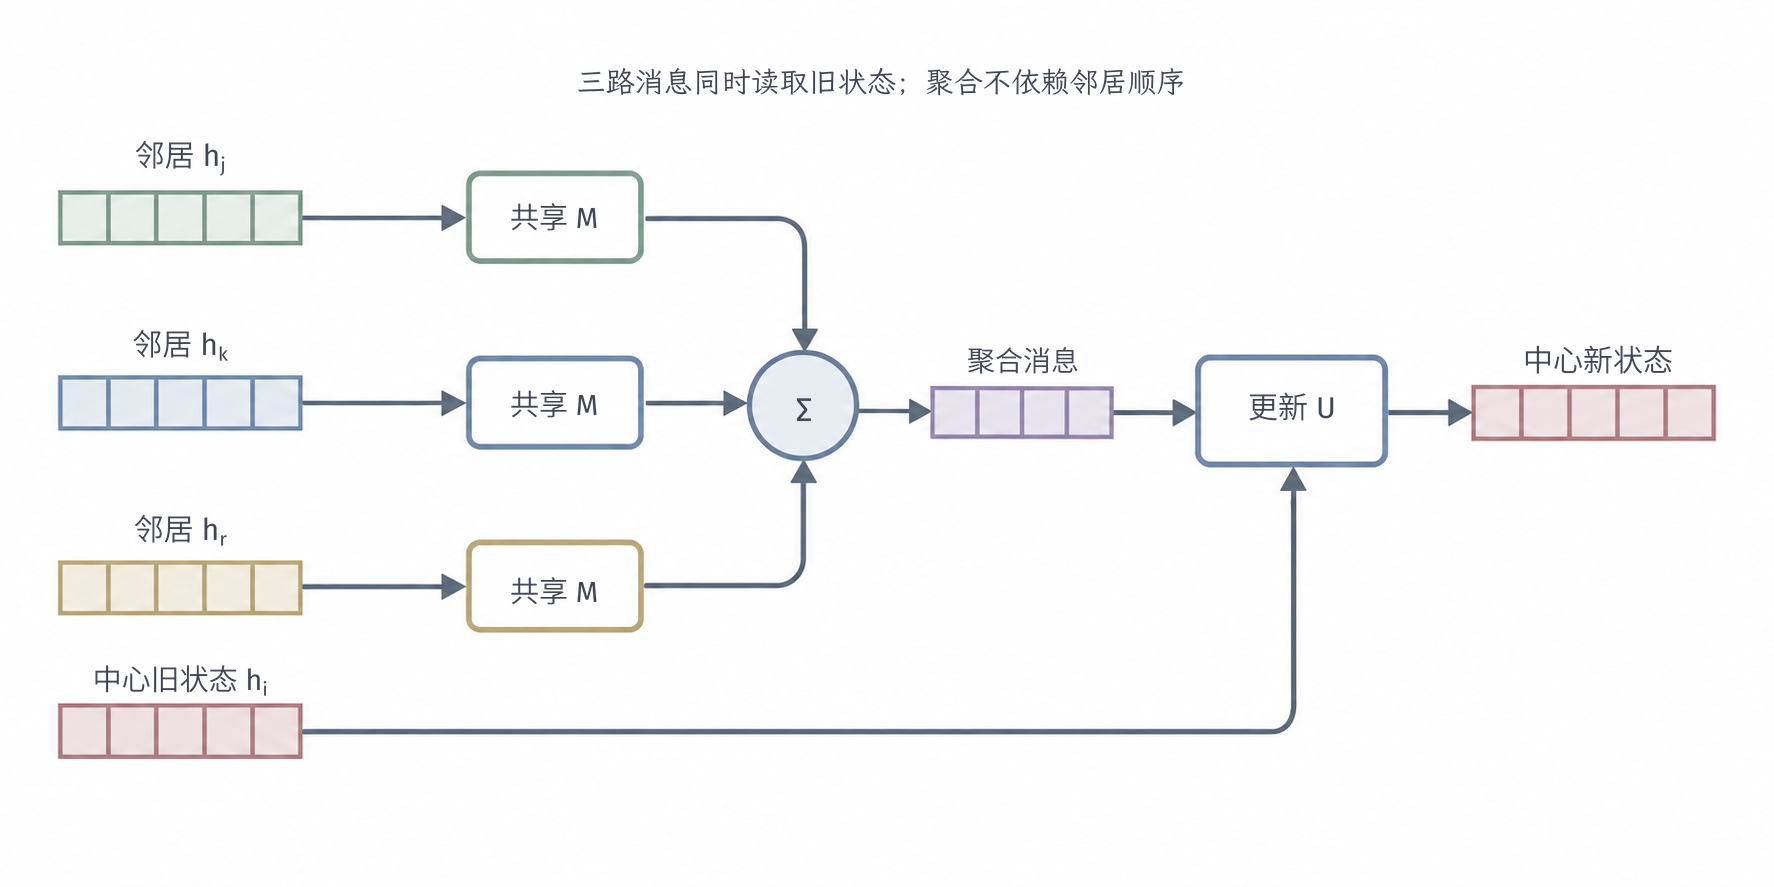
\includegraphics[width=150.199mm]{figures/08-neural-network-models/00-shared/generated/gnn-message-passing/figure.png}
  \caption{节点$i$的一轮消息传递。左侧三行邻居表示分别产生消息，经求和聚合后更新节点$i$。下方独立路径把$i$的旧表示送入更新函数。图中省略消息函数对接收节点和边属性的额外输入，所有节点使用相同的消息与更新规则。}
  \label{fig:gnn-message-passing}
\end{figure*}
\FloatBarrier

在同一轮内，$M^{(l)}$和$U^{(l)}$的参数在所有节点与边上共享。因此，增加节点会增加计算量，却不必增加参数量。若邻域聚合不依赖枚举次序，输入编码和节点更新也使用共享函数，就可按轮归纳证明式\eqref{eq:gnn-permutation}：重编号只重排消息的接收位置，聚合结果跟着重排，更新后的表示也跟着重排。随机邻居采样还要求采样规则与编号无关；不同随机抽样下输出数值未必一致，等变性应针对对应的抽样或输出分布理解。

一轮只能读取直接邻居的旧表示，这正像卷积网络中一层只覆盖一个局部窗口。要让信息传得更远，靠的是\emph{多轮传播}：两轮之后，每个邻居的表示里已经含有它自己邻居的信息，于是当前节点间接看到了两跳之外的节点。\term{图上的感受野}（graph receptive field）就是能够经传播影响当前表示的节点范围；在仅使用一跳邻域、没有全局通路时，$L$轮的范围至多为$L$跳。图~\ref{fig:gnn-propagation}采用同步更新：所有节点都先看上一轮的旧快照、各自算出新快照后再统一替换——这样可以避免“同一轮里先更新的节点被后更新的节点提前看到”，保证一轮最多只能获得一跳的新信息。若改为读取刚更新的状态，传播次序和每轮可见范围都会随之改变。

\begin{figure}[htb]
  \centering
  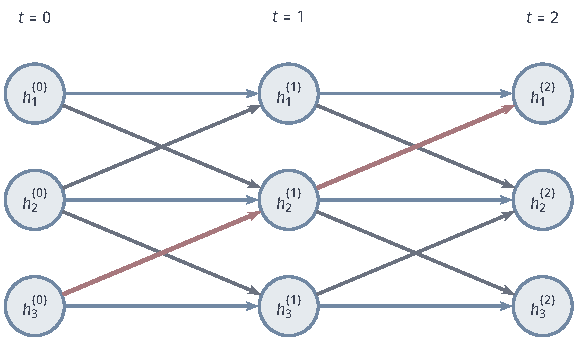
\includegraphics[width=97.794mm]{figures/08-neural-network-models/00-shared/tikz/gnn-propagation/figure.pdf}
  \caption{三节点路径上的同步传播。列顶的$t=0,1,2$表示同步快照，横向实线传递自身状态，斜线沿原图的相邻关系传递状态。红色粗线描出节点3经节点2影响节点1的两跳路径；同一列内没有即时传播，因此一次更新不能直接读取两跳之外的新信息。}
  \label{fig:gnn-propagation}
\end{figure}
\FloatBarrier

\begin{example}[两轮邻域平均]
\label{ex:gnn-two-rounds}
取无向路径$1-2-3$，初始标量为$\bm{x}=(1,0,2)^{\top}$。为单独观察传播，暂不使用可学习参数与非线性，令
\[
  h_i^{(l+1)}=\frac{h_i^{(l)}+\sum_{j\in N(i)}h_j^{(l)}}{1+|N(i)|}\text{。}
\]
一轮结果为$(1/2,1,1)^{\top}$，两轮结果为$(3/4,5/6,1)^{\top}$。节点1在第一轮没有读取节点3，第二轮却通过节点2受到节点3的影响。这是人为构造的传播例子，不是训练所得的实验结果。
\end{example}

节点表示形成后，整图预测还需要\term{读出}（readout）：把数量可变的节点表示变成一个图表示。基本形式是
\begin{equation}
  \bm{g}=\rho\!\left(\sum_{i\in V}\phi(\bm{h}_i^{(L)})\right),
  \qquad \widehat{\bm{y}}=g_{\mathrm{out}}(\bm{g})\text{，}
  \label{eq:gnn-readout}
\end{equation}
其中$\phi$是共享的节点变换，$\rho$是聚合后的变换。求和不因节点重排而改变，所以它把节点等变表示转为整图不变表示。平均会消去部分规模信息，最大值强调是否出现某类特征；若目标随对象数量累积，求和更符合这一结构假设，但仍需验证目标是否具有相应可加性。

只计固定宽度$m$下的稠密线性节点变换和线性消息，一轮常可组织为$O(nm^2+em)$：先对节点变换，再沿边聚合。若每条边都单独通过宽度为$m$的稠密网络，边计算可以达到$O(em^2)$。消息函数的形式和特征宽度共同决定边数的成本系数。保存多轮激活时，训练存储也随节点、边及传播轮次增长；参数共享控制的是参数数目。

\subsection{输出和学习目标}
\label{sec:gnn-output-objectives}

消息传递得到的是每个节点一个表示，但实际要预测的对象可能在三个不同层级：单个节点、一对节点（边）、或整张图。三者可以共用同一个图编码器，区别只在\emph{从哪里读出、用什么损失}。这一区分很重要，因为它决定了是否还能保留节点身份：节点/边任务要求输出与具体位置对应（置换等变），整图任务则必须把所有节点汇成一个与编号无关的量（置换不变）。图~\ref{fig:gnn-output-levels}把这三种读出对应起来；损失函数仍按第~\ref{sec:ffn-output-objectives}节介绍的输出含义选择。

\begin{figure*}[htb]
  \centering
  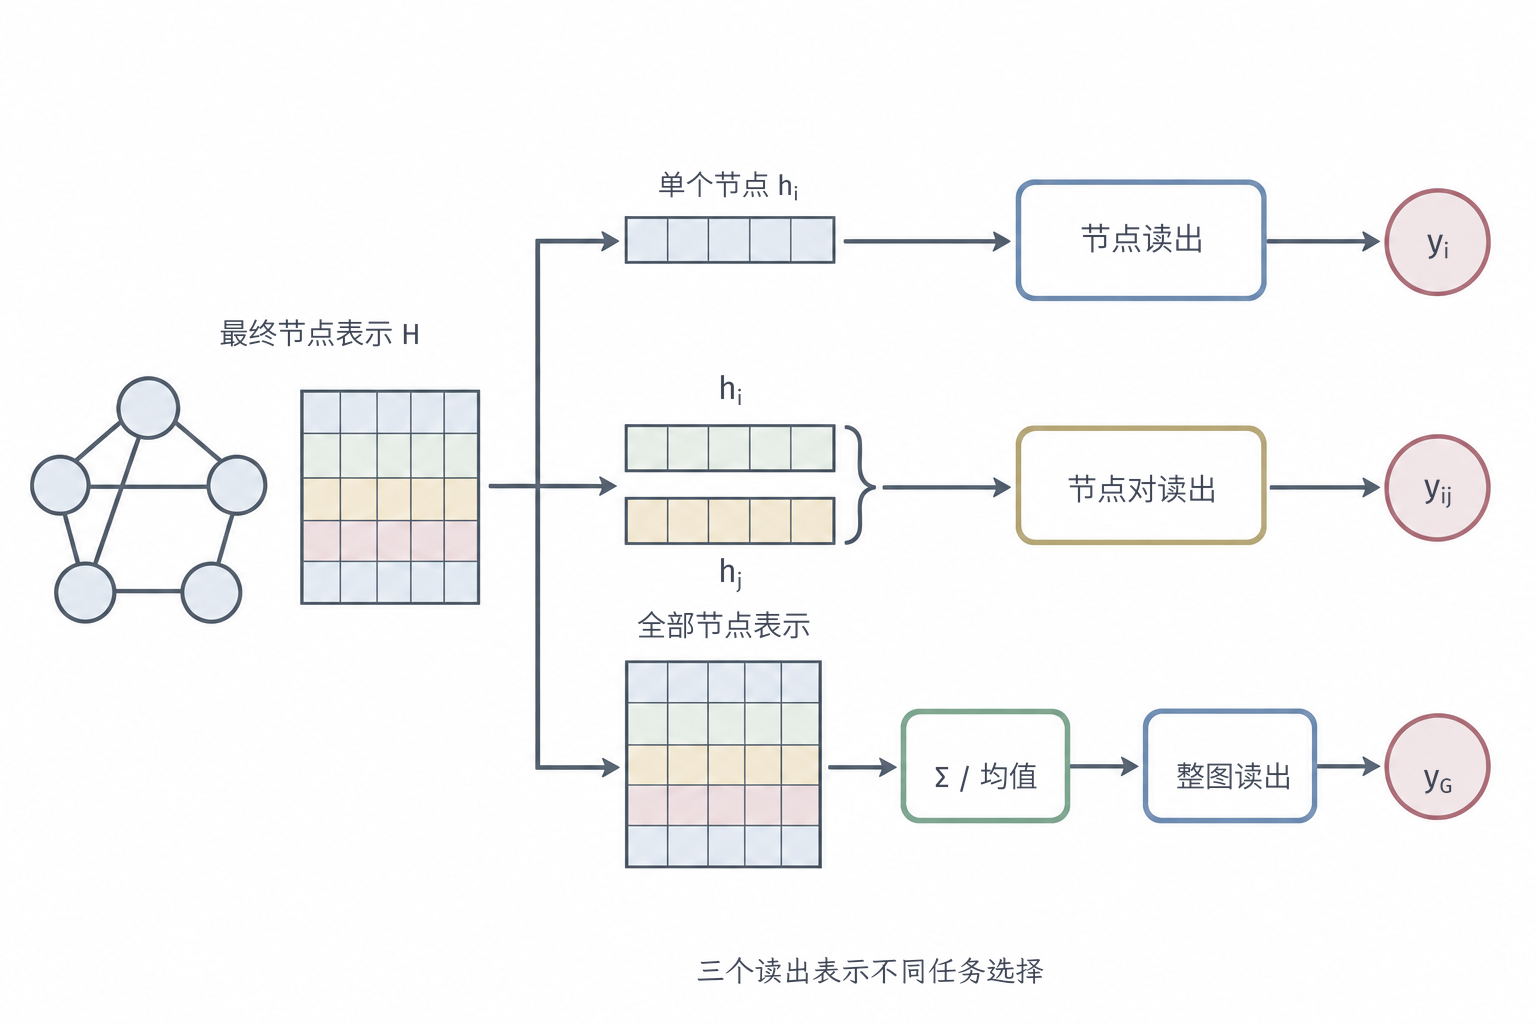
\includegraphics[width=130.048mm]{figures/08-neural-network-models/00-shared/generated/gnn-output-levels/figure.png}
  \caption{同一组节点表示的三种任务读出。三个分支分别承载节点、节点对和整图任务，并在相应位置执行读出。节点预测读取一个节点，边或连接预测读取两个端点及可用的关系属性，整图预测先对全部节点作对称聚合；三个分支不要求在同一模型中同时启用。}
  \label{fig:gnn-output-levels}
\end{figure*}
\FloatBarrier

节点分类在每个受监督节点上计算类别概率。设类别数为$C$，标签$y_i\in\{1,\ldots,C\}$，训练标签所在节点集合为$V_{\mathrm{train}}$，则
\begin{equation}
  \begin{aligned}
    \bm{p}_i&=\operatorname{softmax}(\bm{W}_{\mathrm{out}}\bm{h}_i^{(L)}+\bm{b}_{\mathrm{out}}),\\
    L_{\mathrm{node}}&=-\frac{1}{|V_{\mathrm{train}}|}
      \sum_{i\in V_{\mathrm{train}}}\log p_{i,y_i}\text{。}
  \end{aligned}
  \label{eq:gnn-node-loss}
\end{equation}
$\bm{W}_{\mathrm{out}}\in\mathbb{R}^{C\times m_L}$，$\bm{b}_{\mathrm{out}}\in\mathbb{R}^{C}$。其他节点的可见属性与连接可以按任务设定参加编码，类别标签则放在各自的监督或评估集合中。标签掩码限定哪些节点产生训练损失，输入特征的可见范围由另一个规则确定。

边预测需要同时读取端点。设候选节点对集合为$B$，用成对读出函数计算得分，再变成存在连接的预测概率：
\[
  \begin{aligned}
    s_{i,j}&=g_{\mathrm{pair}}(\bm{h}_i^{(L)},\bm{h}_j^{(L)},\bm{a}_{i,j}),\\
    p_{i,j}&=\operatorname{sigmoid}(s_{i,j})\text{。}
  \end{aligned}
\]
对二值目标$b_{i,j}$可使用
\begin{equation}
  L_{\mathrm{edge}}=-\frac{1}{|B|}\sum_{(i,j)\in B}
    \left[b_{i,j}\log p_{i,j}+(1-b_{i,j})\log(1-p_{i,j})\right]\text{。}
  \label{eq:gnn-edge-loss}
\end{equation}
候选连接尚未被观察到时，可用输入通常只含端点和预测时已知的关系类型，读出据此省略未知边属性。无向连接的评分需要满足$s_{i,j}=s_{j,i}$，例如采用点积；有向连接可以使用一般双线性评分或有序拼接，这类有序评分允许两个方向具有不同得分。

整图预测把第$q$张图的读出$\bm{g}_q$映射为类别或数值，按独立图样本平均损失。回归目标$y_q\in\mathbb{R}$可写为
\begin{equation}
  L_{\mathrm{graph}}=\frac{1}{N}\sum_{q=1}^{N}
    \left(g_{\mathrm{out}}(\bm{g}_q)-y_q\right)^2\text{，}
  \label{eq:gnn-graph-loss}
\end{equation}
其中$N$是训练图数，各图的节点数$n_q$可以不同。记第$q$张图的平方损失为$\ell_q=(g_{\mathrm{out}}(\bm{g}_q)-y_q)^2$，式\eqref{eq:gnn-graph-loss}就是先把各图的$\ell_q$相加，再除以图数$N$，所以每张图的权重都是$1/N$。

如果希望节点更多的图占更大权重，可以改用按节点数加权的整图损失
\[
  L_{\mathrm{graph,node}}=
    \frac{\sum_{q=1}^{N}n_q\ell_q}{\sum_{q=1}^{N}n_q}\text{。}
\]
分子把第$q$张图的损失计入$n_q$次，分母是总节点数，因此该图的权重变为$n_q/\sum_{s=1}^{N}n_s$。这里仍然是每张图产生一个预测和一个损失，并未给各节点另设监督目标。只把式\eqref{eq:gnn-graph-loss}的分母改成总节点数，会同时缩放所有图的损失，不能改变图与图之间的相对权重。

例如，构造两张分别有2个和8个节点的图，令损失分别为1和4。按图平均得到$(1+4)/2=5/2$；按节点数加权得到$(2\times1+8\times4)/(2+8)=17/5$。后一目标给大图的权重是小图的4倍，二者因而对应不同的经验目标。

\Needspace{10\baselineskip}
\subsection{参数学习}
\label{sec:gnn-learning}

\subsubsection{沿消息通路回传梯度}
\label{sec:gnn-message-backprop}

固定$L$轮时，式\eqref{eq:gnn-message-passing}是有限的函数复合。前向沿边$j\to i$读取节点$j$的状态，反向则计算这份状态对节点$i$的预测误差有多大影响，再把相应导数回到$j$。前向读取已经建立这条求导依赖，即使原图没有另设$i\to j$的边，导数仍沿链式法则回到发送者。图中的环已沿传播轮次展开，反向依次处理$l=L-1,\ldots,0$，每次回传都进入更早一轮的状态。

用列向量$\bm{g}_i^{(l)}=\partial L/\partial\bm{h}_i^{(l)}\in\mathbb{R}^{m_l}$记节点状态的总梯度。节点分类的输出头在受监督节点产生初始梯度；整图读出把整图损失回传到参与读出的节点；连接预测的评分头向两个端点回传。没有自身标签的节点也可能因影响其他节点的预测而得到梯度。下面暂设损失只经最终轮状态产生，若中间轮也有输出，须在该轮另加直接损失的导数。

一轮反向计算可以对应前向的三个环节。令消息宽度为$r_l$，聚合宽度为$\overline r_l$，先将$\bm{g}_i^{(l+1)}$经更新函数回到聚合向量，再经聚合回到各条消息：
\begin{equation}
  \begin{aligned}
    \bm{v}_i^{(l)}
      &=\left(\frac{\partial U^{(l)}}
        {\partial\overline{\bm{m}}_i^{(l)}}\right)^{\top}
        \bm{g}_i^{(l+1)},\\
    \bm{\delta}_{i\leftarrow j}^{(l)}
      &=\left(\frac{\partial\operatorname{AGG}^{(l)}}
        {\partial\bm{m}_{i\leftarrow j}^{(l)}}\right)^{\top}
        \bm{v}_i^{(l)}\text{。}
  \end{aligned}
  \label{eq:gnn-message-adjoints}
\end{equation}
这里$\bm{v}_i^{(l)}\in\mathbb{R}^{\overline r_l}$，$\bm{\delta}_{i\leftarrow j}^{(l)}\in\mathbb{R}^{r_l}$；两个局部Jacobian矩阵的形状分别为$m_{l+1}\times\overline r_l$和$\overline r_l\times r_l$。所有导数都在前向保存的状态、消息及参数上计算。求和聚合的Jacobian是单位矩阵，所以每条消息收到同一个$\bm{v}_i^{(l)}$；平均聚合再除以邻居数；逐坐标最大值把导数送到被选中的位置，平局处需约定次梯度或记录规则。内容相关权重也依赖状态，求导时其变化与值向量的变化共同进入梯度。

消息函数的两个状态输入会产生不同贡献。记$\bm{J}_{1,i,j}^{(l)}$、$\bm{J}_{2,i,j}^{(l)}\in\mathbb{R}^{r_l\times m_l}$分别为$M^{(l)}$关于接收端状态和发送端状态的Jacobian。节点$j$的总梯度为
\begin{equation}
  \begin{aligned}
    \bm{g}_j^{(l)}
      &=\left(\frac{\partial U^{(l)}}
        {\partial\bm{h}_j^{(l)}}\right)^{\top}
        \bm{g}_j^{(l+1)}\\
      &\quad+\sum_{i:\,j\in N(i)}
        (\bm{J}_{2,i,j}^{(l)})^{\top}
        \bm{\delta}_{i\leftarrow j}^{(l)}\\
      &\quad+\sum_{k\in N(j)}
        (\bm{J}_{1,j,k}^{(l)})^{\top}
        \bm{\delta}_{j\leftarrow k}^{(l)}\text{。}
  \end{aligned}
  \label{eq:gnn-node-state-gradient}
\end{equation}
第一项经过$j$自身的更新分支，局部偏导把聚合输入暂视为固定；第二项汇总$j$向其他节点发送的消息，正是从各接收节点回到$j$的梯度；第三项来自$j$作为接收端参与消息计算的影响。若消息只依赖发送端，第三项为零。自环使同一状态同时充当两个输入，两个局部贡献都要计入；跨层连接也按其实际计算路径另行累加。

图~\ref{fig:gnn-backpropagation}展示式\eqref{eq:gnn-node-state-gradient}第二项中$i$、$k$两条发送路径的汇合。每条路径先得到消息梯度$\bm\delta_{i\leftarrow j}^{(l)}$或$\bm\delta_{k\leftarrow j}^{(l)}$，再经相应发送端Jacobian的转置，变成对节点$j$状态的贡献。图中把这两份贡献的和记为$\bm g_{j,\mathrm{send}}^{(l)}$；完整的$\bm g_j^{(l)}$还须按该式计入其他发送路径、自身更新和接收端路径。自动微分系统在计算图上完成这种累积；分布式实现若把相关计算放在不同设备上，则需要汇总同一状态和共享参数的贡献。
\begin{figure*}[htb]
  \centering
  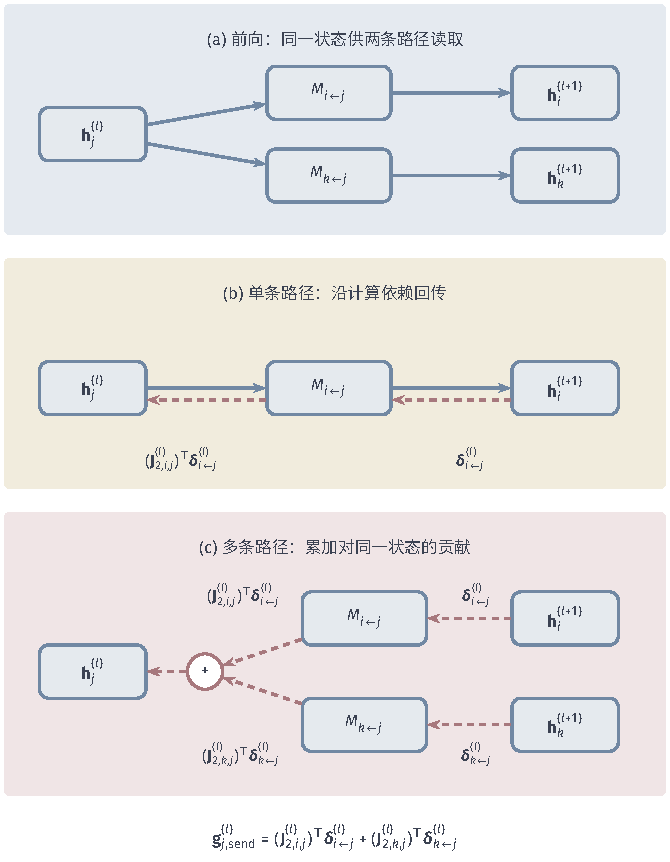
\includegraphics[width=113.404mm]{figures/08-neural-network-models/00-shared/tikz/gnn-backpropagation/figure.pdf}
  \caption{同一节点状态沿两条发送路径收到的梯度贡献。（a）只画前向分叉；（b）跟踪接收节点$i$的回传，消息梯度经发送端Jacobian的转置回到节点$j$；（c）在$+$处累加$i$、$k$两条路径的贡献，记为$\bm g_{j,\mathrm{send}}^{(l)}$。实线表示前向计算，红色虚线表示导数路径。图中贡献和只包含所示的两条发送路径，省略其他消息、自身更新、接收端路径和任务输出头；反向依赖由前向读取决定，不要求原图存在反向边。}
  \label{fig:gnn-backpropagation}
\end{figure*}
\FloatBarrier

状态梯度继续传向上一轮，共享参数的梯度则汇集为本次优化器更新的输入。以一层线性消息$\bm{m}_{i\leftarrow j}=\bm{W}\bm{h}_j$为例，$\bm{W}\in\mathbb{R}^{r_l\times m_l}$，接收端回传的消息梯度给发送端贡献$\bm{W}^{\top}\bm{\delta}_{i\leftarrow j}$，并给权重贡献一个外积。因此
\begin{equation}
  \frac{\partial L}{\partial\bm{W}}
    =\sum_{(j\to i)\in E}
      \bm{\delta}_{i\leftarrow j}\bm{h}_j^{\top}\text{。}
  \label{eq:gnn-shared-gradient}
\end{equation}
跨轮共享$\bm{W}$时，还要对轮次求和。节点更新、输入编码及输出头中的共享参数使用同样规则，正则项的导数另加到相应参数。各边、各轮的贡献汇集后，优化器更新这一份共享权重。

\begin{example}[无标签节点怎样得到梯度]
\label{ex:gnn-unlabeled-gradient}
沿用示例~\ref{ex:gnn-two-rounds}的两轮平均，只在节点1设置目标0，取$L=\tfrac12(h_1^{(2)})^2$。此处状态与梯度都是标量，记$g_i^{(l)}=\partial L/\partial h_i^{(l)}$。由$h_1^{(2)}=3/4$，最终轮梯度为$(3/4,0,0)$。节点1的第二轮输出平均了上一轮节点1和2的状态，故
\[
  \bm{g}^{(1)}=(3/8,3/8,0)^{\top},\qquad
  \bm{g}^{(0)}=(5/16,5/16,1/8)^{\top}\text{。}
\]
例如节点3没有标签，却通过节点2影响节点1；它在初始轮收到的梯度为$(3/8)\times(1/3)=1/8$。由于$h_3^{(0)}=x_3$，这个数值是损失$L$对初始属性$x_3$的导数。

预测量$h_1^{(2)}$对同一输入的导数需要单独区分。节点3的初始属性先以系数$1/3$进入$h_2^{(1)}$，再以系数$1/2$进入$h_1^{(2)}$，所以
\[
  \frac{\partial h_1^{(2)}}{\partial x_3}
    =\frac12\times\frac13=\frac16,\qquad
  \frac{\partial L}{\partial x_3}
    =\frac{\partial L}{\partial h_1^{(2)}}
      \frac{\partial h_1^{(2)}}{\partial x_3}
    =\frac34\times\frac16=\frac18\text{。}
\]
前者衡量预测对输入属性的敏感度；后者还计入当前预测与目标0的偏差$3/4$，衡量的是损失的敏感度。这里没有可学习的传播参数，例子只核对状态及输入的导数；当前任务更新的参数范围仍由模型定义。
\end{example}

\subsubsection{训练批次与信息范围}
\label{sec:gnn-training-batches}

图训练有一个前几章没有的特殊问题：计算一个节点的表示，需要它的邻居，而邻居又需要它们的邻居……那么训练时到底要载入多大一片图？几种做法对应不同的信息范围和计算代价，需要先分清。

\term{全图训练}（full-graph training）在每次前向计算中读取完整的训练可见图，再只在受监督的位置计算损失。单图节点分类时可以只抽取一批标签位置，却仍要计算全图的节点表示——这与只读取部分结构的训练不同。若手上是许多独立小图（如一批分子），可以用块对角邻接矩阵把它们拼成一张互不连通的大图统一计算，读出时再按图归属分别聚合，保证一个分子的节点不会“看到”另一个分子。

大图上$L$跳邻域会随层数指数膨胀（一个高度数节点的邻居的邻居很快就覆盖大半张图），全图计算的显存和时间都可能不可承受。\term{邻居采样}（neighbor sampling）为本批目标节点逐层只随机选取有限个邻居，在采出的计算图上前向和反向：每层最多取$s$个邻居时，未经去重的展开规模约为$1+s+\cdots+s^L$。采样限制了每个节点的分支数，但多层递推仍会逐层展开这些分支。需要注意一个常被忽略的偏差问题：均匀采样的均值可以无偏估计\emph{一次固定的}邻域平均，但非线性更新之后，“先采样再过网络”的预测及其梯度通常\emph{不再}是全图结果的无偏估计；归一化和多层抽样会进一步改变计算。

\term{子图训练}（subgraph training）则直接抽取一部分节点及其边，在这张子图内完成多轮传播。它便于让多个目标节点共享中间计算，但截断边界会丢掉来自外围的消息；若希望完整保留目标节点的$L$跳邻域，可以把外围节点作为上下文纳入。采样误差、边界缺失和标签抽样是三种不同的误差来源，不能混为一谈。

数据的\emph{可见范围}还取决于任务设定，这直接影响训练是否“合法”。\term{直推学习}（transductive learning）针对训练时就已存在的一批对象预测其未知标签：例如引用网络的全部结构和论文特征在训练时都可见，只是部分节点不给标签——测试节点的特征和连接可以参与前向编码，唯独不用它们的标签。\term{归纳学习}（inductive learning）则要求把规则用到训练时\emph{从未见过}的新节点或新图上（如给刚发表的论文、新增的分子分类）。共享消息函数两种设定都适用，因为参数随对象复用是计算结构的性质；但二者评估的泛化能力不同，必须用对应的数据划分来检验。

无论哪种设定，每次更新都应明确三件事：可见图是哪些、输入特征可见到什么程度、监督集合包含谁。对连接预测，还必须在编码图中移除待评估的目标边及其副本（否则模型直接“读到”了要预测的连接，等于漏题）；对动态预测，结构和属性只能来自预测时刻之前。

\subsubsection{参数更新与收敛条件}
\label{sec:gnn-optimization-convergence}

反向传播给出当前参数下的导数，优化器才决定怎样改变参数。将全部可学习参数记为$\bm{\theta}\in\mathbb{R}^{p}$，固定数据与可见图，记训练损失加正则项为$J(\bm{\theta})$。一次普通梯度更新为
\begin{equation}
  \bm{\theta}^{(t+1)}=\bm{\theta}^{(t)}
    -\eta_t\widehat{\bm{g}}^{(t)}\text{，}
  \label{eq:gnn-parameter-update}
\end{equation}
$t$是优化器更新次数，与传播轮次$l$不同；$\eta_t>0$是学习率。全目标求导时$\widehat{\bm{g}}^{(t)}=\nabla J(\bm{\theta}^{(t)})$，抽批次时则是相应计算得到的梯度估计。同一次更新的前向和反向使用同一份参数。旧梯度累积按训练规则清除或保留，本批贡献再求和或按约定平均，随后进入优化器。

网络的多层复合、消息函数和输出头通常使$J$非凸。训练进展可以由损失值、梯度尺度或参数变化测量；达到驻点与找到全局最小值又有不同的条件。共享参数与归一化会改变目标及传播尺度，求解保证仍需由完整优化问题建立。

一个有条件的结果说明梯度法为什么可能稳定降低目标。假定$J$有下界$J_{\inf}$，且梯度是$\beta$-Lipschitz的，即$\lVert\nabla J(\bm{u})-\nabla J(\bm{v})\rVert_2\leq\beta\lVert\bm{u}-\bm{v}\rVert_2$，其中$\beta>0$。沿连接两参数的线段积分梯度，可得
\[
  J(\bm{u})\leq J(\bm{v})+
  \langle\nabla J(\bm{v}),\bm{u}-\bm{v}\rangle
  +\frac{\beta}{2}\lVert\bm{u}-\bm{v}\rVert_2^2\text{。}
\]
若使用完整梯度与固定学习率$0<\eta\leq1/\beta$，代入式\eqref{eq:gnn-parameter-update}即得到
\begin{equation}
  \begin{aligned}
    J(\bm{\theta}^{(t+1)})
      &\leq J(\bm{\theta}^{(t)})
        -\frac{\eta}{2}\lVert\nabla J(\bm{\theta}^{(t)})\rVert_2^2,\\
    \min_{0\leq t<T}\lVert\nabla J(\bm{\theta}^{(t)})\rVert_2^2
      &\leq\frac{2[J(\bm{\theta}^{(0)})-J_{\inf}]}{\eta T}\text{。}
  \end{aligned}
  \label{eq:gnn-gradient-descent-bound}
\end{equation}
第二行由第一行对$T$次更新求和得到，$T$是优化步数。它控制前若干次更新中最小的梯度范数平方；在这些假设下，各迭代点的梯度范数也趋于零。参数序列是否有极限、驻点是否全局最优，还需进一步条件。ReLU与最大聚合具有不可微位置，实际目标的有限平滑常数$\beta$也需要在所分析区域建立，光滑结论的适用范围由此确定。

抽样梯度还增加了波动。若它在给定参数下无偏、方差有统一上界，并满足相应光滑性及下界条件，递减学习率可以控制梯度噪声。经典条件包括$\sum_t\eta_t=\infty$和$\sum_t\eta_t^2<\infty$，能保证按学习率加权的期望梯度平方范数平均值趋于零。这个指标描述迭代过程的加权平均，参数极限与全局最优另需条件。固定非零学习率通常只能保证平均梯度大小受噪声项控制，单步损失不必持续下降。Bottou等的分析明确区分了这两种情形\scite{bottou2018optimization} 在固定编码图上，均匀抽取标签位置并按目标正确缩放，可以保持完整标签平均损失的无偏梯度；邻居采样经过多层非线性却未必如此。标签抽样和邻域抽样可能对应不同梯度对象，收敛分析随实际目标和更新规则确定；自适应优化器也需要对应的条件。

实际停止可结合最大步数、在固定评估计算上的训练损失与梯度范数，以及验证指标的早停。传播深度、初始化、度归一化、残差与门控会影响链式Jacobian的尺度，从而影响梯度过小或过大的程度；学习率和优化器也须与该尺度匹配。可以据实际梯度和目标变化检验这些设计对训练条件的影响。固定参数下的状态迭代是否收敛则是另一问题，第~\ref{sec:gnn-state-convergence}节讨论其充分条件；新对象上的误差则由匹配预测设定的数据另行检验。

\section{卷积图神经网络}
\label{sec:gnn-convolutional}

消息传递已经能处理任意图，但“每个节点用什么权重聚合邻居”仍可进一步设计。本章标题中的“图卷积”，指的是把第3章卷积网络在规则网格上\emph{共享滤波系数}的思想推广到不规则图：在图像上，每个位置都用同一组核系数，因为“右边一格”在任何位置含义相同；图上没有统一的相对坐标，节点的邻居不仅数量不同、没有次序，编号差也不代表距离。于是“卷积”在图上必须重新定义——它不再对应一个滑动窗口，而是一个\emph{作用在图信号上的共享传播算子}。

这种推广有两个互补的思考入口，初学时可以分别理解、最终会合到同一处。
\begin{itemize}
  \item \textbf{谱域入口}沿用信号处理中“卷积定理”的形式：先把节点上的信号分解成若干种振荡模式（图的傅里叶基），在模式空间里逐分量缩放，再变换回来。它在数学上优雅，但要先求出整张图的特征向量，计算昂贵且难以跨图迁移。
  \item \textbf{空域入口}沿用消息传递的直觉：沿每个节点的邻域，用同一套规则组合邻居、再做与次序无关的聚合。它直观、稀疏、易扩展。
\end{itemize}
\term{图卷积}（graph convolution）正是这两者的统称；本节会看到，当谱域滤波器取为拉普拉斯的多项式时，两个入口在数学上完全等价——\emph{在频率空间设计滤波器，等价于在节点邻域上做有限跳的稀疏传播}。一般图缺少网格上的统一平移，因此“卷积”由图关系上的算子定义，再由该算子决定传播行为和计算代价。

一个线性图滤波器可以把两种入口联系起来。令$\bm{Q}\in\mathbb{R}^{n\times n}$是给定的局部传播矩阵，非对角非零元只位于相邻节点间；邻接矩阵就是一个选择。对$\bm{H}\in\mathbb{R}^{n\times d_{\mathrm{in}}}$，可定义
\begin{equation}
  \bm{Z}=\sum_{k=0}^{K}\bm{Q}^{k}\bm{H}\bm{W}_k,
  \qquad \bm{W}_k\in\mathbb{R}^{d_{\mathrm{in}}\times d_{\mathrm{out}}}\text{。}
  \label{eq:gnn-polynomial-convolution}
\end{equation}
其中$\bm{Q}^0=\bm{I}_n$，$\bm{Z}\in\mathbb{R}^{n\times d_{\mathrm{out}}}$；$k=0$处理自身，$k\geq1$组织至多$k$跳内经传播到达的信息。$\bm{W}_k$在所有节点共享，并不为每条具体路径另设参数。计算时递推$\bm{H}_0=\bm{H}$、$\bm{H}_k=\bm{Q}\bm{H}_{k-1}$，累加$\bm{H}_k\bm{W}_k$，无需显式形成通常更稠密的$\bm{Q}^k$。非线性激活再作用于$\bm{Z}$，多层这样的计算构成网络。

式\eqref{eq:gnn-polynomial-convolution}如何包含普通卷积，可以在周期的一维有向网格上看清。取移位矩阵$\bm{T}$，满足$(\bm{T}\bm{x})_i=x_{i-1}$，下标按周期返回；则单通道有限核的循环卷积是$\sum_{r=-K}^{K}w_r\bm{T}^{r}\bm{x}$。不同偏移对应重复移位或反向移位。一般图改用邻接或拉普拉斯等关系算子组织传播。单个无向对称算子把两方向按同一关系处理；带方向或类型差别的核则需要相应的关系信息及不同的关系算子。

共享还必须服从重编号。若$\bm{Q}'=\bm{P}\bm{Q}\bm{P}^{\top}$、$\bm{H}'=\bm{P}\bm{H}$，则$\bm{Z}'=\bm{P}\bm{Z}$，因为$(\bm{P}\bm{Q}\bm{P}^{\top})^k\bm{P}=\bm{P}\bm{Q}^k$。这使局部组合不依赖节点保存次序。但一般消息传递比线性卷积更广：注意力或非线性边消息可以让权重依赖输入，不必对应某个固定的线性频率响应。下面分别从图信号的模式与邻域计算定义具体算子，再比较两者的联系和适用条件。

\subsection{谱域图神经网络}
\label{sec:gnn-spectral}

\subsubsection{图拉普拉斯与图傅里叶变换}
\label{sec:gnn-graph-fourier}

要理解谱域图卷积，先回答“图上的频率是什么”。把每个节点上的一个标量看成图信号，直觉上：如果相邻节点的取值都差不多（信号在边上变化平缓），这是\emph{低频}成分；如果相邻节点取值剧烈跳变（信号在每条边上都在振荡），这是\emph{高频}成分。图拉普拉斯正是一个度量“相邻差异总和”的算子，它可以把任意信号分解成从平缓到剧烈的一系列正交模式；本节要学习的是如何对不同模式施加不同的响应（比如平滑去噪就保留低频、抑制高频）。

记$d_i=\sum_j\bm A_{i,j}$为节点度，$\bm D=\operatorname{diag}(d_1,\ldots,d_n)$为度矩阵。
节点度差异较大时，常用\term{对称归一化拉普拉斯}（symmetric normalized Laplacian），以免高度数节点主导一切。
本节为简化推导，假定所有节点$d_i>0$，令
\begin{equation}
  \bm{L}=\bm{I}_n-\bm{D}^{-1/2}\bm{A}\bm{D}^{-1/2}
    =\bm{U}\bm{\Lambda}\bm{U}^{\top}\text{。}
  \label{eq:gnn-laplacian-spectrum}
\end{equation}
$\bm{U}\in\mathbb{R}^{n\times n}$的列$\bm{u}_k$是正交特征向量，$\bm{\Lambda}$的对角元素$\lambda_k\in[0,2]$按升序排列。归一化后的能量比较$x_i/\sqrt{d_i}$与$x_j/\sqrt{d_j}$，因此零频模式在每个连通分量内与$\sqrt{d_i}$成比例，未必是常量；不同分量可以具有不同的比例系数。图连通时，零特征空间才只有这一个方向。存在孤立节点时须另规定归一化约定，或加自环后再定义相应算子。

在当前归一化拉普拉斯的图傅里叶坐标$\widehat{\bm x}=\bm U^\top\bm x$中，
让频率响应$g_{\bm\theta}(\lambda)$随训练参数改变，得到可学习的谱滤波：
\begin{equation}
  \bm{y}=\bm{U}g_{\bm{\theta}}(\bm{\Lambda})\bm{U}^{\top}\bm{x}
    =g_{\bm{\theta}}(\bm{L})\bm{x}\text{。}
  \label{eq:gnn-spectral-filter}
\end{equation}
图~\ref{fig:gnn-spectral-filter}显示这三步。谱域图卷积沿用傅里叶域逐模式相乘的形式；图的连接决定这些模式，所以滤波的含义由图谱而非普通空间偏移给出。

\begin{figure*}[htb]
  \centering
  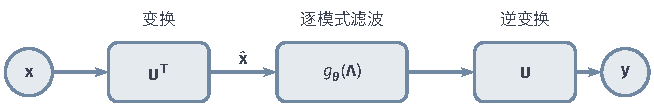
\includegraphics[width=110.793mm]{figures/08-neural-network-models/00-shared/tikz/gnn-spectral-filter/figure.pdf}
  \caption{谱滤波的计算路径。节点信号$\bm{x}$经$\bm{U}^{\top}$分解为图傅里叶系数，每个模式由$g_{\bm{\theta}}(\lambda_k)$调整，再经$\bm{U}$还原为节点信号。左、右两端使用同一张图和同一节点顺序；中间向量的下标表示频率模式。}
  \label{fig:gnn-spectral-filter}
\end{figure*}
\FloatBarrier

\begin{example}[三节点路径上的低频模式]
\label{ex:gnn-low-frequency}
沿用路径$1-2-3$，此处不加自环，度为$(1,2,1)$。归一化拉普拉斯的特征值为$0,1,2$，可取
\[
  \bm{u}_1=\tfrac12(1,\sqrt2,1)^{\top},\quad
  \bm{u}_2=\tfrac{1}{\sqrt2}(1,0,-1)^{\top},\quad
  \bm{u}_3=\tfrac12(1,-\sqrt2,1)^{\top}\text{。}
\]
输入$\bm{x}=(1,0,2)^{\top}$的三个系数为$3/2,-1/\sqrt2,3/2$。若只保留零频模式，输出为$(3/4,3\sqrt2/4,3/4)^{\top}$。中间节点的数值较大，恰是度归一化后的平滑，而不是普通算术平均。
\end{example}

\subsubsection{Spectral CNN：直接学习频率响应}
\label{sec:gnn-spectral-cnn}

Bruna等的Spectral CNN把谱滤波放入多通道网络。对输入通道$a$与输出通道$b$，可以学习一个对角滤波器$\bm{\Theta}_{a,b}$，用$\bm{U}\bm{\Theta}_{a,b}\bm{U}^{\top}$变换对应信号，再累加通道并使用非线性。完整谱上的自由响应需要每通道对$n$个参数；原工作还用少量样条系数插值得到平滑响应，减少参数自由度\scite{bruna2014spectral}

固定图与傅里叶基时，前向计算是矩阵乘法，滤波参数可按链式法则求导。例如单通道$\bm{y}=\bm{U}\operatorname{diag}(\bm{\theta})\widehat{\bm{x}}$，上游梯度为$\bm{v}=\partial L/\partial\bm{y}$，则$\partial L/\partial\theta_k=(\bm{U}^{\top}\bm{v})_k\widehat x_k$。通道与样本之间共享参数时，对相应贡献求和即可。

直接使用稠密$\bm{U}$需要$O(n^2)$的单信号变换和存储，完整稠密特征分解的常规代价为$O(n^3)$。只保留部分特征向量可以改变代价，但也限制了可用模式。自由频率响应还可能对应全图稠密算子，读取范围要由实际响应检验；有限跳数局部性需要另加结构。

对新图，特征值与特征向量都会变化，按旧图谱索引学习的自由系数没有自然的一一对应。特征向量的符号在$\bm{U}\bm{\Theta}\bm{U}^{\top}$中相消，但重特征值对应的子空间还可以旋转；若该子空间内使用不同自由系数，算子就依赖具体基的选择。由同一个标量函数$g(\lambda)$定义响应，能够消除这种基选择歧义；跨图迁移的预测效果仍需另行验证。

\subsubsection{ChebNet：用多项式实现局部滤波}
\label{sec:gnn-chebnet}

Spectral CNN虽然给了图卷积一个干净的谱定义，却有两个致命的工程问题：要显式求出并保存稠密的特征基$\bm U$（代价$O(n^3)$、存储$O(n^2)$），而且这些基是\emph{针对某一张具体的图}算出来的——在一张引用图上学到的频率系数，换一张结构不同的图就无处对齐，无法迁移。解决思路来自信号处理中的一个事实：\emph{如果让频率响应$g$是拉普拉斯矩阵$\bm L$的多项式，那么$g(\bm L)\bm x$根本不需要显式的$\bm U$，只用稀疏的矩阵—向量乘法就能算}；而且多项式系数只描述“怎么对$\bm L$组合”，可以直接拿到另一张图上用它自己的$\bm L$重新计算。ChebNet用\term{切比雪夫多项式}（Chebyshev polynomial）来参数化这个响应，既有良好的数值性质又能控制阶数。设$\lambda_*>0$是拉普拉斯谱的上界，令$\widetilde{\bm{L}}=2\bm{L}/\lambda_*-\bm{I}_n$，把谱放到$[-1,1]$；归一化拉普拉斯可取$\lambda_*=2$。约定$K$为最高次数，则
\begin{equation}
  g_{\bm{\theta}}(\bm{L})\bm{x}
    =\sum_{k=0}^{K}\theta_k T_k(\widetilde{\bm{L}})\bm{x}\text{，}
  \label{eq:gnn-chebyshev-filter}
\end{equation}
其中$T_0(z)=1$、$T_1(z)=z$、$T_k(z)=2zT_{k-1}(z)-T_{k-2}(z)$。有些文献用$K$表示项数，此时最高次数为$K-1$，阅读时须核对约定\scite{defferrard2016chebnet}

令$\bm{z}_k=T_k(\widetilde{\bm{L}})\bm{x}$，即可用$\bm{z}_0=\bm{x}$、$\bm{z}_1=\widetilde{\bm{L}}\bm{x}$以及$\bm{z}_k=2\widetilde{\bm{L}}\bm{z}_{k-1}-\bm{z}_{k-2}$递推。整个过程只需要稀疏矩阵乘向量；单通道的$K\geq1$阶计算量为$O(K(n+e))$，无需构造$\bm{U}$。反向传播也经过这些稀疏乘法，系数梯度为$\bm{v}^{\top}\bm{z}_k$。

多项式为何局部，可以从矩阵乘法看出。$\bm{L}$的非对角非零元只连接相邻节点，一次相乘至多走一条边；$\bm{L}^k$至多连接$k$跳以内。故式\eqref{eq:gnn-chebyshev-filter}在一层中读取至多$K$跳邻域。多通道形式为$\bm{Y}=\sum_{k=0}^{K}T_k(\widetilde{\bm{L}})\bm{X}\bm{\Theta}_k$，$\bm{\Theta}_k\in\mathbb{R}^{d_{\mathrm{in}}\times d_{\mathrm{out}}}$，参数量为$(K+1)d_{\mathrm{in}}d_{\mathrm{out}}$，不随$n$增加。

这些系数描述同一个多项式，所以可以在另一张图上重新构造拉普拉斯并使用它们，无需对齐特征向量。频率分布与任务关系随图改变，预测质量也需在新图上检验。若使用的谱上界过小，使缩放后的特征值落到$[-1,1]$以外，高次多项式还可能迅速放大误差。

\subsection{空域图神经网络}
\label{sec:gnn-spatial}

ChebNet已经把谱卷积化成了邻域上的稀疏传播，空域方法则干脆直接在消息传递框架里设计聚合规则，不再借助傅里叶语言。下面四个经典模型可以理解为针对同一个朴素邻域平均的四次“挑刺”，每个解决一个具体缺陷：GCN解决\emph{度数不均导致的尺度问题}（用归一化加权而非简单平均），GraphSAGE解决\emph{大图算不动、新节点无法归纳}的问题（采样+拼接自身），GAT解决\emph{归一化权重与内容无关}的问题（按邻居相关性动态加权），GIN则解决\emph{平均/最大聚合会丢掉邻居数量差异}的表达能力问题（用求和保多重集）。它们共享前面的输出与反向传播机制，主要差别只在聚合和更新两步。

\subsubsection{GCN：归一化的邻域传播}
\label{sec:gnn-gcn}

先看最简单的邻域平均会有什么问题。直接把自己和所有邻居的特征相加，度数很高的节点（一个连了上千邻居的枢纽）聚合出的数值会远大于度数低的节点，数值尺度随度数剧烈波动，训练难以稳定。\term{图卷积网络}（graph convolutional network, GCN）在本节特指Kipf与Welling提出的层形式，它的核心就是一个\emph{按两端度数归一化}的传播矩阵：加入自环$\widetilde{\bm{A}}=\bm{A}+\bm{I}_n$（让节点也读取自身），令$\widetilde d_i=\sum_j\widetilde{\bm{A}}_{i,j}$，定义
\begin{equation}
  \bm{S}=\widetilde{\bm{D}}^{-1/2}\widetilde{\bm{A}}\widetilde{\bm{D}}^{-1/2},
  \qquad
  \bm{H}^{(l+1)}=\sigma\!\left(\bm{S}\bm{H}^{(l)}\bm{W}^{(l)}\right)\text{。}
  \label{eq:gnn-gcn-layer}
\end{equation}
$\bm{H}^{(l)}\in\mathbb{R}^{n\times m_l}$按行存放状态，$\bm{H}^{(0)}=\bm{X}$；$\bm{W}^{(l)}\in\mathbb{R}^{m_l\times m_{l+1}}$变换特征通道，$\sigma$逐坐标作用。采用行存放的矩阵形式时，节点列向量的变换对应$(\bm{W}^{(l)})^{\top}\bm{h}_i^{(l)}$。原始层式省略偏置，增加共享偏置不会改变置换等变性。

从节点$j$到$i$的消息系数为$\widetilde{\bm{A}}_{i,j}/\sqrt{\widetilde d_i\widetilde d_j}$，同时计入边权以及接收端与发送端的度。边权为1时，才简化为$1/\sqrt{\widetilde d_i\widetilde d_j}$。这个组合按两端度归一化；$\bm{S}$的行和未必等于1，数值因此不同于算术平均。沿用三节点无权路径与输入$(1,0,2)^{\top}$，取单位特征变换和恒等激活，得到
\begin{equation}
  \bm{S}=\begin{pmatrix}
    1/2&1/\sqrt6&0\\
    1/\sqrt6&1/3&1/\sqrt6\\
    0&1/\sqrt6&1/2
  \end{pmatrix},\qquad
  \bm{S}\bm{x}=\begin{pmatrix}1/2\\3/\sqrt6\\1\end{pmatrix}\text{。}
  \label{eq:gnn-gcn-example}
\end{equation}
这一结果与示例~\ref{ex:gnn-two-rounds}的平均不同，差别来自归一化规则。

它与谱域方法的联系可以直接推导。对不加自环的归一化拉普拉斯，ChebNet取$K=1$及$\lambda_*=2$时，$\widetilde{\bm{L}}=-\bm{D}^{-1/2}\bm{A}\bm{D}^{-1/2}$。再约束$\theta_0=-\theta_1=\theta$，得到$\theta(\bm{I}_n+\bm{D}^{-1/2}\bm{A}\bm{D}^{-1/2})\bm{x}$。GCN进一步以加自环后重新计算度的$\bm{S}$替换括号内算子，限制反复传播的尺度。这一步更换了传播算子及其度归一化；原论文称其为重新归一化技巧\scite{kipf2017gcn}

固定结构时，GCN的梯度也可写清。记$\bm{Z}=\bm{S}\bm{H}\bm{W}$，$\bm{\Delta}=\partial L/\partial\bm{Z}$，则
\begin{equation}
  \frac{\partial L}{\partial\bm{W}}=(\bm{S}\bm{H})^{\top}\bm{\Delta},\qquad
  \frac{\partial L}{\partial\bm{H}}=\bm{S}^{\top}\bm{\Delta}\bm{W}^{\top}\text{。}
  \label{eq:gnn-gcn-backprop}
\end{equation}
激活的导数已并入$\bm{\Delta}$。不学习邻接关系时，$\bm{S}$作为给定算子；学习边权或建图规则时，才需进一步计算结构相关梯度。

标准GCN直接混合相邻节点的变换特征。相邻对象与预测目标相关时，这种共享聚合可以提供有用信息；相邻节点常具有不同标签或关系语义时，混合也可能损失区分所需的特征。共享权重可以接新图重建的传播算子；归纳表现需要按照新图的信息范围和数据检验，原始实验设定只说明其当时的任务。

\subsubsection{GraphSAGE：采样并学习邻域组合}
\label{sec:gnn-graphsage}

GCN仍有两个适用边界：它一次要读取每个节点的\emph{全部}邻居，在百万节点的大图上为一批目标节点展开完整邻域代价过高；而且它的计算依赖整张固定的图，遇到训练后才新加入的节点就无法直接套用（不支持归纳）。GraphSAGE的改造有两点：一是每轮只\emph{随机采样}固定数量的邻居，把计算量钉死；二是把“自身表示”和“邻居聚合结果”先\emph{分开}再拼接，让网络用不同权重分别决定保留多少自身信息、吸收多少邻域信息。这样新节点到达时，只要按相同规则采样其邻居、读取可用属性即可生成表示，而不必依赖它在训练图中的编号。以平均聚合为例，从$N(i)$中取$S_i^{(l)}$，令
\begin{equation}
  \begin{aligned}
    \bm{u}_i^{(l)}&=\frac{1}{|S_i^{(l)}|}\sum_{j\in S_i^{(l)}}\bm{h}_j^{(l)},\\
    \bm{h}_i^{(l+1)}&=\sigma\!\left(
      \bm{W}^{(l)}[\bm{h}_i^{(l)};\bm{u}_i^{(l)}]+\bm{b}^{(l)}\right)\text{。}
  \end{aligned}
  \label{eq:gnn-graphsage}
\end{equation}
分号表示向量拼接，此处$\bm{W}^{(l)}\in\mathbb{R}^{m_{l+1}\times2m_l}$。自身和邻居先分开，再由不同的权重块组合；原算法还可对输出作$\ell_2$归一化，零向量需要单独处理\scite{hamilton2017graphsage}

聚合器也可对邻居先作共享前馈变换，再取逐坐标最大值。平均保留总体水平，最大池化突出某种响应是否出现。原论文还试验了对随机邻居顺序使用LSTM的聚合器。一次LSTM输出取决于所抽顺序；对称聚合直接消除枚举次序，随机顺序方案则需说明对称化或输出分布的口径。

训练时采样所需邻域，计算节点或关系任务的损失，联合更新聚合器、组合矩阵及输出头。预测新节点时沿相同规则读取可用特征与邻域，不必为它单独学习一个节点编号嵌入。新节点可提供的属性与邻域决定表示的信息来源。只使用旧节点编号时，可迁移属性不足；新节点缺乏特征或邻居时也需要相应初态或补充输入。

\subsubsection{GAT：根据内容调整邻居权重}
\label{sec:gnn-gat}

GCN的归一化权重只由图的\emph{拓扑}（各节点的度）决定：一旦图固定，某个邻居占多大权重就固定了，与邻居当前的特征、与当前任务是否相关完全无关。但直觉上，聚合时理应更重视\emph{内容上更相关}的邻居。\term{图注意力网络}（graph attention network, GAT）借用第4章的注意力思想：用节点特征临时为每条边计算一个权重，再在图约束的可见邻域内归一化加权——注意这里的可见范围仍由边严格限定（不是任意两节点都能注意），这是它与Transformer自注意力的关键区别。对一个注意力头，令$\bm{z}_i=\bm{W}\bm{h}_i$，其中$\bm{W}\in\mathbb{R}^{m'\times m}$，则
\begin{equation}
  \begin{aligned}
    e_{i,j}&=\operatorname{LeakyReLU}
      \!\left(\bm{a}^{\top}[\bm{z}_i;\bm{z}_j]\right),\\
    \alpha_{i,j}&=\frac{\exp(e_{i,j})}
      {\sum_{k\in N(i)\cup\{i\}}\exp(e_{i,k})},\\
    \bm{h}'_i&=\sigma\!\left(\sum_{j\in N(i)\cup\{i\}}
      \alpha_{i,j}\bm{z}_j\right)\text{。}
  \end{aligned}
  \label{eq:gnn-gat}
\end{equation}
$\bm{a}\in\mathbb{R}^{2m'}$是共享评分参数；$e_{i,j}$是标量得分，与本章的边数$e$不同。Softmax只在节点$i$的可见邻域内归一化，所有节点使用同一评分函数，所以邻居重排只重排对应权重\scite{velickovic2018gat}

多头注意力分别学习变换和评分，在隐藏层拼接结果，或在输出层取平均。训练时梯度同时通过值向量和权重；若把权重当作常量，就漏掉了评分函数对损失的影响。固定每头宽度时，增加头数还会增加总宽度和参数量，相同宽度预算下的比较需相应分配各头维度。

与前章的循环注意力一样，GAT把“计算权重”和“读取信息”分开；区别是可见位置由图的邻接关系约束。原始GAT的评分使用线性拼接，若将$\bm{a}$拆成两部分，得分是单调激活作用于一个接收端项与一个发送端项之和。因此，在固定候选邻居特征下，邻居排序不能仅靠改变接收端特征任意翻转。这说明原始评分虽随内容产生权重，候选排序仍受到该加性结构的限制。

注意力调整可见邻居之间的相对影响，单轮读取范围仍由图限定。归一化权重描述一次聚合中的数值比例，预测作用还取决于表示内容、评分变化及后续计算；解释或因果结论需要另外的证据。

\subsubsection{GIN：保留邻域多重集合的差别}
\label{sec:gnn-gin}

前几种模型默认用平均（或最大）聚合，但前面强调过，多重集合里\emph{元素的重复次数是信息}；平均和最大恰恰会系统性地抹掉这种计数差别。考虑两个邻域：$\{\!\{1,1\}\!\}$（两个邻居都取1）与$\{\!\{1,1,1\}\!\}$（三个邻居都取1），它们的平均都是1、最大也都是1——度数不同这个事实在聚合后彻底消失。再如$\{\!\{0,2\}\!\}$与$\{\!\{1,1\}\!\}$，连求和都相同（都等于2）。要区分这些结构，必须先选用能保留计数的聚合（求），再配足够灵活的特征映射把和中混在一起的差异分开。图~\ref{fig:gnn-aggregation}展示第一种信息损失。

\begin{figure*}[htb]
  \centering
  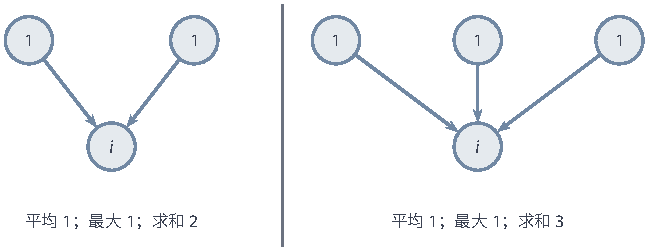
\includegraphics[width=109.792mm]{figures/08-neural-network-models/00-shared/tikz/gnn-aggregation/figure.pdf}
  \caption{聚合如何保留或丢掉重复次数。两个邻域分别含两个和三个数值为1的邻居。平均与最大值都产生1，求和分别产生2和3。图只比较固定标量消息；求和本身也不能区分所有不同多重集合，还需要合适的特征映射。}
  \label{fig:gnn-aggregation}
\end{figure*}
\FloatBarrier

\term{图同构网络}（graph isomorphism network, GIN）使用求和聚合与前馈更新：
\begin{equation}
  \bm{h}_i^{(l+1)}=\operatorname{MLP}^{(l)}\!\left(
    (1+\epsilon^{(l)})\bm{h}_i^{(l)}
      +\sum_{j\in N(i)}\bm{h}_j^{(l)}\right)\text{，}
  \label{eq:gnn-gin}
\end{equation}
$\epsilon^{(l)}$可以固定或学习，用于区分中心节点与邻居的贡献。参数通过任务损失反向传播；整图读出还可拼接各层节点求和，保留不同传播范围的信息\scite{xu2019gin}

比较两张图时，若存在保持连接关系及给定属性的节点重编号，使两图相互对应，就称它们\term{同构}（isomorphic）。GIN的区分能力通过下面的标记更新检验作比较。衡量其区分能力的一种参照是\term{一维Weisfeiler--Leman检验}（1-dimensional Weisfeiler--Leman test, 1-WL）：从与节点属性一致的初始标记出发，反复用“节点旧标记及邻居标记的多重集合”产生新标记。所比较的图必须使用同一套无冲突标记规则，相同的输入组合得到相同标记，不同组合得到不同标记。每轮比较两图全部节点标记组成的多重集合；只要有一轮不同，就可判为非同构，始终相同时，检验仍留下未判定的图对。

对于只使用节点状态、对称邻域聚合且不引入额外区分信息的消息传递网络，1-WL无法区分的图也不能靠这些更新与节点多重集合读出区分：同标记节点具有同样的邻域标记多重集合，共享计算遂逐轮产生同样的状态。

在可数特征域、邻域大小有界，以及聚合、更新和读出满足相应单射性条件时，求和特征映射可以达到1-WL的区分能力。\term{单射}（injective）表示不同输入不会被映成同一个结果。有限宽度和训练得到的映射，需要按实际输入检查前述特征域与单射条件。

1-WL本身也有边界。六节点环与两个互不连接的三角形都具有六个节点，每个节点度为2。若初始节点特征全部相同，这两张图上的节点在每轮都会收到两个相同状态，任何上述消息传递加节点多重集合读出都无法区分它们。共同的两邻居模式随轮次持续重复，单靠更多轮数仍无法区分。子结构信息、更高阶状态或其他任务输入可以改变这类区分条件；由数据学得的预测质量还由训练与泛化分析评价。

\subsection{谱域与空域的联系、区别及选择}
\label{sec:gnn-spectral-spatial-comparison}

谱域与空域的区别主要在于怎样规定算子，而不是计算一定发生在哪一类存储空间。谱域用$g_{\bm{\theta}}(\lambda)$规定不同变化模式的响应，空域用邻居的选择、消息和聚合规定局部组合。若$g_{\bm{\theta}}$是多项式，$\bm{U}g_{\bm{\theta}}(\bm{\Lambda})\bm{U}^{\top}$等于同一多项式作用于$\bm{L}$，便可完全通过节点域稀疏传播计算。ChebNet由谱域设计、按邻域递推实现，GCN也保留了谱域推导。谱域规定响应，节点域稀疏传播实现它；同一模型由此可以同时具有频率与局部邻域解释。

表~\ref{tab:gnn-spectral-spatial}将显式谱实现与多项式实现分开。比较计算量时固定一张稀疏图与单通道线性传播，不计特征通道变换、消息网络及初次特征分解的代价；任意空域消息网络的成本还取决于其具体函数。
\begin{table*}[htb]
  \centering
  \small
  \begin{tabularx}{\linewidth}{@{}p{17mm}XXX@{}}
    \toprule
    比较方面 & 显式谱基滤波 & 多项式谱滤波 & 局部空域聚合\\
    \midrule
    算子定义 & 在图傅里叶模式上规定响应 & 用低阶多项式参数化响应 & 用邻居消息、权重及更新规定组合\\
    实际计算 & $\bm{U}^{\top}$、对角滤波、$\bm{U}$ & 拉普拉斯的稀疏乘法递推 & 沿可见边计算，再按节点聚合\\
    局部范围 & 自由响应通常涉及全图 & $K$次多项式至多读取$K$跳 & 一轮通常读取一跳；可另加长程边\\
    传播成本 & 稠密基下$O(n^2)$ & $O(K(n+e))$ & 一跳简单聚合为$O(n+e)$\\
    跨图使用 & 按旧谱索引的自由参数缺少自然对应 & 共享多项式系数，在新图重建算子 & 共享消息规则，在新图读取邻域\\
    \bottomrule
  \end{tabularx}
  \caption{谱域与空域图卷积的比较。显式谱基滤波表示直接使用完整图傅里叶基的实现；多项式谱滤波同时具有有限邻域解释。跨图使用一行只说明计算规则能否复用，不能据此保证新图上的预测效果。}
  \label{tab:gnn-spectral-spatial}
\end{table*}
\FloatBarrier

在大图、多个大小不同的图或不断变化的图上，直接依赖完整$\bm{U}$有几项实际困难。特征分解与稠密变换占用时间和存储，图结构改变后还需处理新的谱；按某张图谱索引学习的系数无法直接对应另一张图的模式。一般自由响应又不是严格局部的，一批目标节点可能依赖大量其他节点，难以只取少量邻居完成同一计算。这些条件解释了为何直接使用完整特征基的早期实现较少成为大规模局部模型的计算方式。

沿边的空域计算容易与邻居采样及小批次结合，也便于让消息读取边类型、方向和接收端内容。复杂度在稀疏图与固定宽度下可随边数增长，参数不必随节点数增加。这种组织便于局部计算，优化和信息保留还取决于消息、深度和数据。多项式谱滤波也能绕开显式特征分解、共享局部传播；它与自由谱基实现的成本和读取范围分别比较。

完整谱基、多项式滤波和空域聚合提供了不同的计算取舍，选择时应回到所需关系。若关心图信号哪些频率应保留或抑制，谱响应提供了直接的设计和分析对象；若需要不同边类型、内容相关交互或采样邻域，空域消息规则更便于表达这些计算。固定线性滤波、有限邻域与跨图复用可以同时成立；输入相关的非线性消息则未必是单个固定谱滤波器。比较两类网络时，应同时写清算子定义、实际实现、可见范围和数据条件。

谱滤波的后续研究继续改进参数化与计算方式。2022年的ChebNetII通过切比雪夫插值组织可学习的谱响应，改进原有滤波器的参数化\scite{he2022chebnetii} 2026年的L2G-NET研究图傅里叶变换的结构化分解，用子图谱表示及其组合处理局部与全局信息，针对完整谱变换的成本和局部性提出新的计算方式\scite{fernandez2026l2gnet} 这些工作进一步探索了频率响应、局部传播和全局交互之间的联系，各自的收益需要结合任务与数据检验。

\section{循环图神经网络}
\label{sec:gnn-recurrent}

前面的GCN、GAT等模型为每一“层”学习一组不同参数：第1层和第2层做的是不同变换。但还可以有另一种设计哲学：如果“在图上反复传播并融合邻居信息”这件事本身值得做很多次，为什么每一轮都要用不同的规则？循环图网络让\emph{同一套更新规则在同一张固定的图上反复作用}，像第4章的RNN在时间上共享参数一样，这里在传播轮次上共享参数。务必先澄清一个易混点：本节的“轮次”是算法内部的迭代次数，\emph{图本身并不随轮次改变}（输入始终是同一张图）；现实中随时间演化的动态图是另一回事，在第~\ref{sec:gnn-dynamic}节处理。

\subsection{网络结构}
\label{sec:gnn-recurrent-structure}

\term{循环图神经网络}（recurrent graph neural network）在同一图上反复更新所有节点的隐状态，直到满足停止条件或达到预定轮数。将全部状态按节点堆成列向量$\bm{h}^{(t)}\in\mathbb{R}^{nm}$，令参数向量为$\bm{\theta}\in\mathbb{R}^{p}$，可写为
\begin{equation}
  \bm{h}^{(t+1)}=F_{\bm{\theta}}(\bm{h}^{(t)};\mathcal{G},\bm{X}),
  \qquad \widehat{\bm{y}}=g_{\bm{\theta}}(\bm{h}^{(T)})\text{。}
  \label{eq:gnn-recurrent-update}
\end{equation}
$F_{\bm{\theta}}$内部仍包含共享消息、聚合与节点更新；分号后的图与属性在各轮固定。图~\ref{fig:gnn-recurrent}显示同一规则的多次调用，每次调用的状态值不同。跨轮共享还要求相应状态维度兼容。

\begin{figure*}[htb]
  \centering
  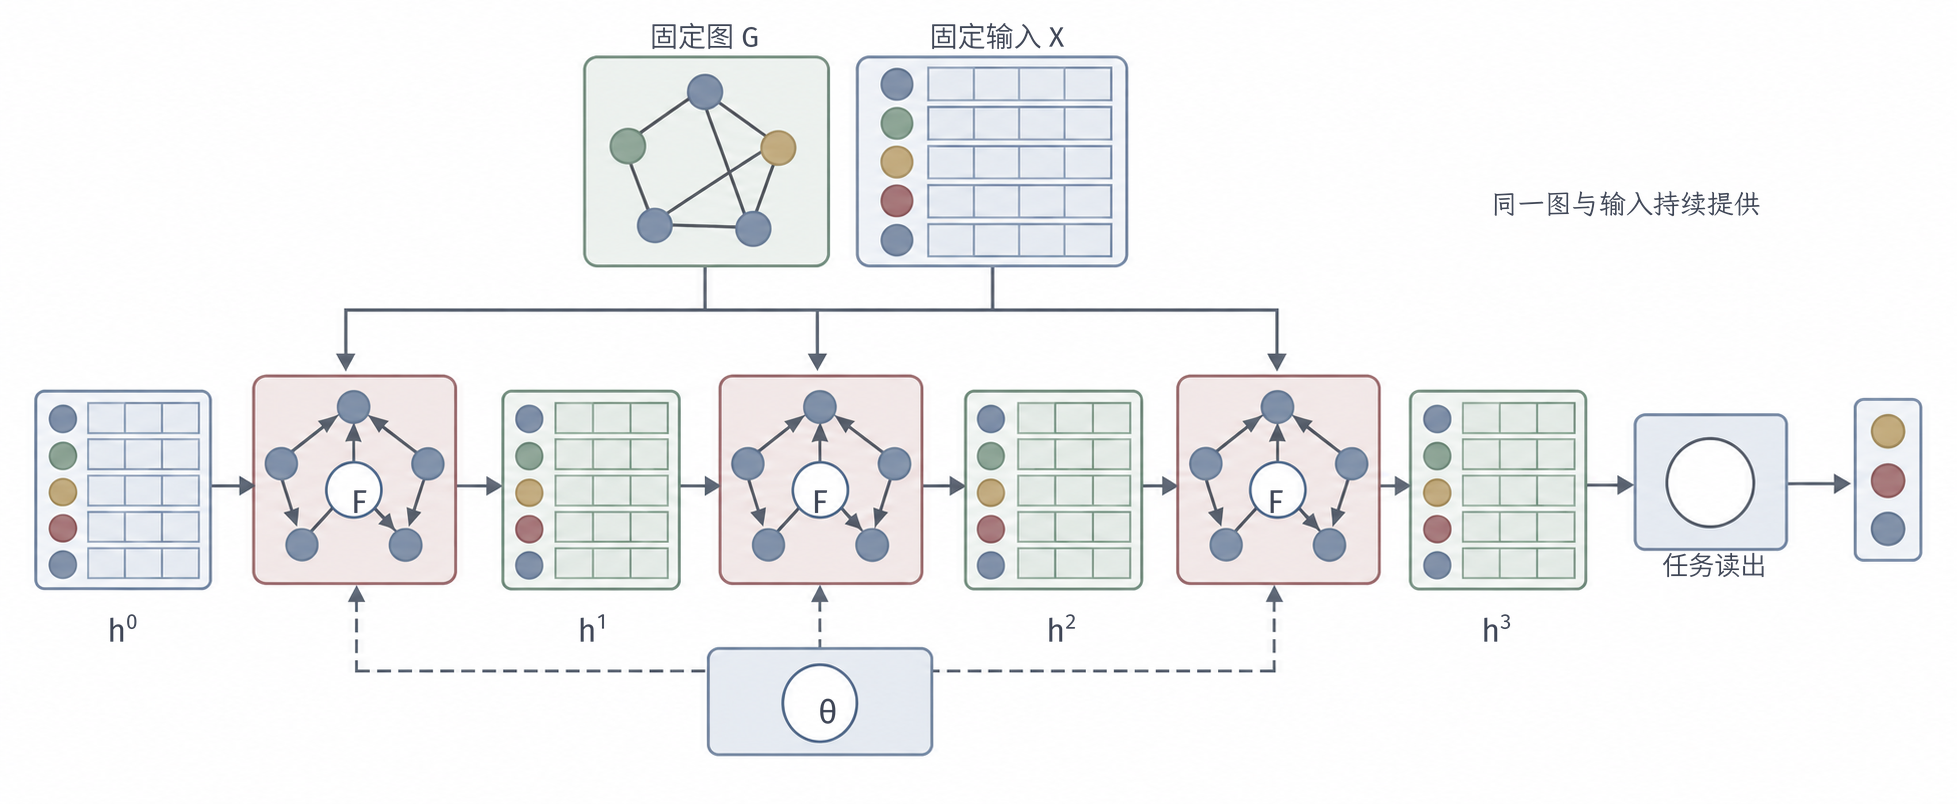
\includegraphics[width=165.693mm]{figures/08-neural-network-models/00-shared/generated/gnn-recurrent/figure.png}
  \caption{固定图上的循环更新。左侧表示邻接关系，右侧展开三轮共享更新$F_{\bm{\theta}}$，每个状态向量包含整张图的节点状态。固定图与输入特征在各轮重复供给，状态沿轮次传递，任务读出从最终状态形成预测。轮次是内部计算步，不表示图已经发生三个时间点的变化。}
  \label{fig:gnn-recurrent}
\end{figure*}
\FloatBarrier

共享参数使每轮复用同一规则，执行代价仍累加各轮计算。状态更新和任务监督决定传播内容；若目标是最短路或关系推理，还需检验这些表示与目标规则的对应。有限轮次模型与迭代至稳定的模型分别定义不同的输出。

\subsection{典型模型}
\label{sec:gnn-recurrent-models}

\subsubsection{以不动点为目标的图网络}
\label{sec:gnn-fixed-point-model}

早期GNN把目标状态定义为\term{不动点}（fixed point）：再次使用更新函数后仍不改变的状态，即$\bm{h}^*=F_{\bm{\theta}}(\bm{h}^*;\mathcal{G},\bm{X})$。它通过邻居状态迭代计算这一表示，再读取节点或图输出。为保证状态可确定，模型约束更新对状态具有收缩性；第~\ref{sec:gnn-state-convergence}节的状态收敛分析将给出条件及误差界。

这类模型的参数既影响输出映射，也影响不动点的位置。有限精度计算通常在相邻两轮差小于容差时停止，并设置最大轮数。达到轮数上限时输出当前近似状态，与容差已满足的情况分别记录。所需精度、迭代成本和收缩约束共同决定这一表示怎样求得。

\subsubsection{GGNN：固定轮次的门控传播}
\label{sec:gnn-ggnn}

如果任务只需要执行有限步，可以直接学习这些步骤的结果。\term{门控图神经网络}（gated graph neural network, GGNN）在聚合后用GRU式更新保留或写入状态。令$r(i,j)$表示边的类型与方向，邻域输入为
\begin{equation}
  \bm{a}_i^{(t)}=\sum_{j\in N(i)}\bm{W}_{r(i,j)}\bm{h}_j^{(t-1)}+\bm{b},
  \qquad
  \bm{h}_i^{(t)}=\operatorname{GRU}(\bm{h}_i^{(t-1)},\bm{a}_i^{(t)})\text{。}
  \label{eq:gnn-ggnn}
\end{equation}
这里$\bm{a}_i^{(t)}$是聚合输入向量，与边属性$\bm{a}_{i,j}$通过索引形式区分。原模型分别处理入边与出边并组合相应消息；式\eqref{eq:gnn-ggnn}写出一个统一的关系聚合形式，方向也可编码为不同类型\scite{li2016ggnn}

GRU的门机制沿用第~\ref{sec:rnn-gru}节。若把更新门解释为写入比例，状态可写为$\bm{h}_i^{(t)}=(\bm{1}-\bm{z}_i^{(t)})\odot\bm{h}_i^{(t-1)}+\bm{z}_i^{(t)}\odot\widetilde{\bm{h}}_i^{(t)}$；候选状态同时依赖聚合输入与经重置门处理的旧状态。门为节点提供选择性保留路径，远处证据则仍须沿边经过足够轮次。

GGNN用预先设定的$T$轮展开计算并训练，输出定义为第$T$轮状态，无需把它作为不动点近似。有限展开放宽了早期模型的收缩约束，状态行为由这些实际步骤决定。训练轮数是模型的一部分；预测时增加轮次就改变了所执行的函数，需要相应检验。

\subsection{参数学习}
\label{sec:gnn-recurrent-learning}

有限展开的梯度与随时间反向传播具有相同结构。设局部状态Jacobian矩阵$\bm{J}^{(t)}=\partial\bm{h}^{(t+1)}/\partial\bm{h}^{(t)}$，$\bm{\delta}^{(t)}$为第$t$轮状态的总梯度。若损失只读取末状态，则$\bm{\delta}^{(t)}=(\bm{J}^{(t)})^{\top}\bm{\delta}^{(t+1)}$；中间轮存在直接监督时，另加对应梯度。共享更新参数的梯度为
\begin{equation}
  \nabla_{\bm{\theta}}L
    =\left.\nabla_{\bm{\theta}}L\right|_{\mathrm{direct}}
      +\sum_{t=0}^{T-1}(\bm{B}^{(t)})^{\top}\bm{\delta}^{(t+1)}\text{，}
  \label{eq:gnn-recurrent-gradient}
\end{equation}
其中$\bm{B}^{(t)}=\partial F_{\bm{\theta}}(\bm{h}^{(t)};\mathcal{G},\bm{X})/\partial\bm{\theta}$固定当前输入状态求偏导。直接项包含读出参数等依赖；初态若依赖参数，还需计入初态梯度。截断展开会遗漏更早的间接贡献，降低存储与计算的同时改变所用梯度。

不动点模型还可用\term{隐式微分}（implicit differentiation）：对定义状态的方程求导，而不保存全部前向迭代。假设更新在不动点附近可微，令$\bm{J}_*=\partial F/\partial\bm{h}$、$\bm{B}_*=\partial F/\partial\bm{\theta}$在$\bm{h}^*$处取值。若$\bm{I}-\bm{J}_*$可逆，则
\begin{equation}
  (\bm{I}-\bm{J}_*)\frac{\partial\bm{h}^*}{\partial\bm{\theta}}
    =\bm{B}_*\text{。}
  \label{eq:gnn-implicit-state-gradient}
\end{equation}
这个等式来自对$\bm{h}^*=F_{\bm{\theta}}(\bm{h}^*)$两侧求导，并把状态导数项移到左侧。

实际需要的是标量损失的梯度。记$\bm{v}=\partial L/\partial\bm{h}^*\in\mathbb{R}^{nm}$为列向量，$\bm{D}_*=\partial\bm{h}^*/\partial\bm{\theta}\in\mathbb{R}^{nm\times p}$为状态对参数的导数矩阵。链式法则给出的状态间接项是$\bm{D}_*^{\top}\bm{v}$；若直接求出整个$\bm{D}_*$，就要为$p$个参数方向分别求状态响应。标量损失只需要这些响应在$\bm{v}$方向上的组合，因此可以先求一个$nm$维向量$\bm{u}$，再将它映回参数空间。具体地，解下面的转置线性方程，并用$\bm{B}_*^{\top}\bm{u}$计算间接项：
\begin{equation}
  (\bm{I}-\bm{J}_*^{\top})\bm{u}=\bm{v},\qquad
  \nabla_{\bm{\theta}}L
    =\left.\nabla_{\bm{\theta}}L\right|_{\mathrm{direct}}+\bm{B}_*^{\top}\bm{u}\text{。}
  \label{eq:gnn-implicit-loss-gradient}
\end{equation}
这一替换可以直接由两个线性关系核对。式\eqref{eq:gnn-implicit-state-gradient}给出$(\bm{I}-\bm{J}_*)\bm{D}_*=\bm{B}_*$，转置线性方程则给出$\bm{v}=(\bm{I}-\bm{J}_*)^{\top}\bm{u}$，所以
\[
  \begin{aligned}
    \bm{D}_*^{\top}\bm{v}
      &=\bm{D}_*^{\top}(\bm{I}-\bm{J}_*)^{\top}\bm{u}\\
      &=\bigl((\bm{I}-\bm{J}_*)\bm{D}_*\bigr)^{\top}\bm{u}
       =\bm{B}_*^{\top}\bm{u}\text{。}
  \end{aligned}
\]
直接项仍是在固定$\bm{h}^*$时，损失经读出等路径对参数产生的导数。这样只需解一个状态空间中的转置线性系统，无需形成整个状态导数矩阵。

无需显式求逆。若相应范数下$\lVert\bm{J}_*\rVert<1$，可用$\bm{u}^{(k+1)}=\bm{v}+\bm{J}_*^{\top}\bm{u}^{(k)}$迭代；Jacobian转置与向量的乘积由自动微分计算。前向状态与后向线性求解都有容差，两者都会影响最终梯度的精度。

对只迭代到近似状态的模型，有限展开给出实际执行步骤的梯度，隐式方法近似理想不动点目标的梯度，二者在尚未充分收敛时未必相同。停止条件、最大轮数和状态收缩速度因而既影响前向代价，也影响参数学习。

\section{图神经网络的扩展}
\label{sec:gnn-extensions}

前面的消息传递默认了几件事：所有边语义相同、图静止不变、一次关系只涉及两个节点、节点没有几何坐标。现实关系往往打破这些假设：论文之间“引用”和“合著”含义不同（多关系），社交网络随时变化（动态），一次合作涉及多人（高阶），分子中的原子还带三维坐标且预测要尊重旋转平移（几何）。扩展模型的共同原则是：把这些额外差异\emph{显式保留在输入里}，并设计相应的消息和对称约束，而不是让它们在无差别的聚合中被抹掉。

\subsection{多关系与异构图}
\label{sec:gnn-relational}

此前所有边都被当成同一种关系，但“甲引用乙”和“甲与乙合著”传递的是完全不同的信息，用同一套权重混合会把语义差别抹掉。\term{多关系图}（multi-relational graph）允许边带有类型，让不同类型的消息走不同的变换；\term{异构图}（heterogeneous graph）进一步允许节点本身分属不同类型（作者、论文）、具有不同属性和角色。节点类型与边类型是两个独立的分类维度，可以单独指定，也可以同时存在。

设关系类型集合为$R$，$N_r(i)$是通过类型$r$向$i$发送消息的邻居。\term{关系图卷积网络}（relational graph convolutional network, R-GCN）为每种关系使用一组独立变换：
\begin{equation}
  \bm{h}_i^{(l+1)}=\sigma\!\left(
    \bm{W}_0^{(l)}\bm{h}_i^{(l)}+
    \sum_{r\in R}\sum_{j\in N_r(i)}
      \frac{1}{c_{i,r}}\bm{W}_r^{(l)}\bm{h}_j^{(l)}\right)\text{。}
  \label{eq:gnn-rgcn}
\end{equation}
$c_{i,r}>0$是归一化系数，可在非空邻域取$|N_r(i)|$；空邻域的求和直接为零。$\bm{W}_0^{(l)}$负责自身状态，$\bm{W}_r^{(l)}$负责关系$r$。有向关系可增加单独的逆关系类型，使两个方向使用不同参数\scite{schlichtkrull2018rgcn}

关系数很大时，每种关系独立学习一个稠密矩阵会增加参数与数据需求。可以用基分解$\bm{W}_r=\sum_{b=1}^{B}a_{r,b}\bm{V}_b$，让各关系共享$B$个基础矩阵，只学习不同系数。固定输入输出宽度$m$时，参数量由$|R|m^2$改为$Bm^2+|R|B$，代价是关系变换被限制在同一矩阵子空间。

不同节点类型的原始特征维度可能不同，可以先用类型相关的输入映射投到公共空间，再按关系传递。聚合还可先在每种关系内部组合，再学习关系间权重。置换等变性在重编号后仍成立，但类型也须跟着节点与边重排。作者和论文的属性角色保持各自含义，重编号只改变保存它们的位置。

图~\ref{fig:gnn-typed-relations}用作者与论文两类节点说明这种分工。类型映射先对齐特征空间，关系变换与归一化随后保留“撰写”和“引用”的区别，自身状态仍有独立路径。

\begin{figure*}[htbp]
  \centering
  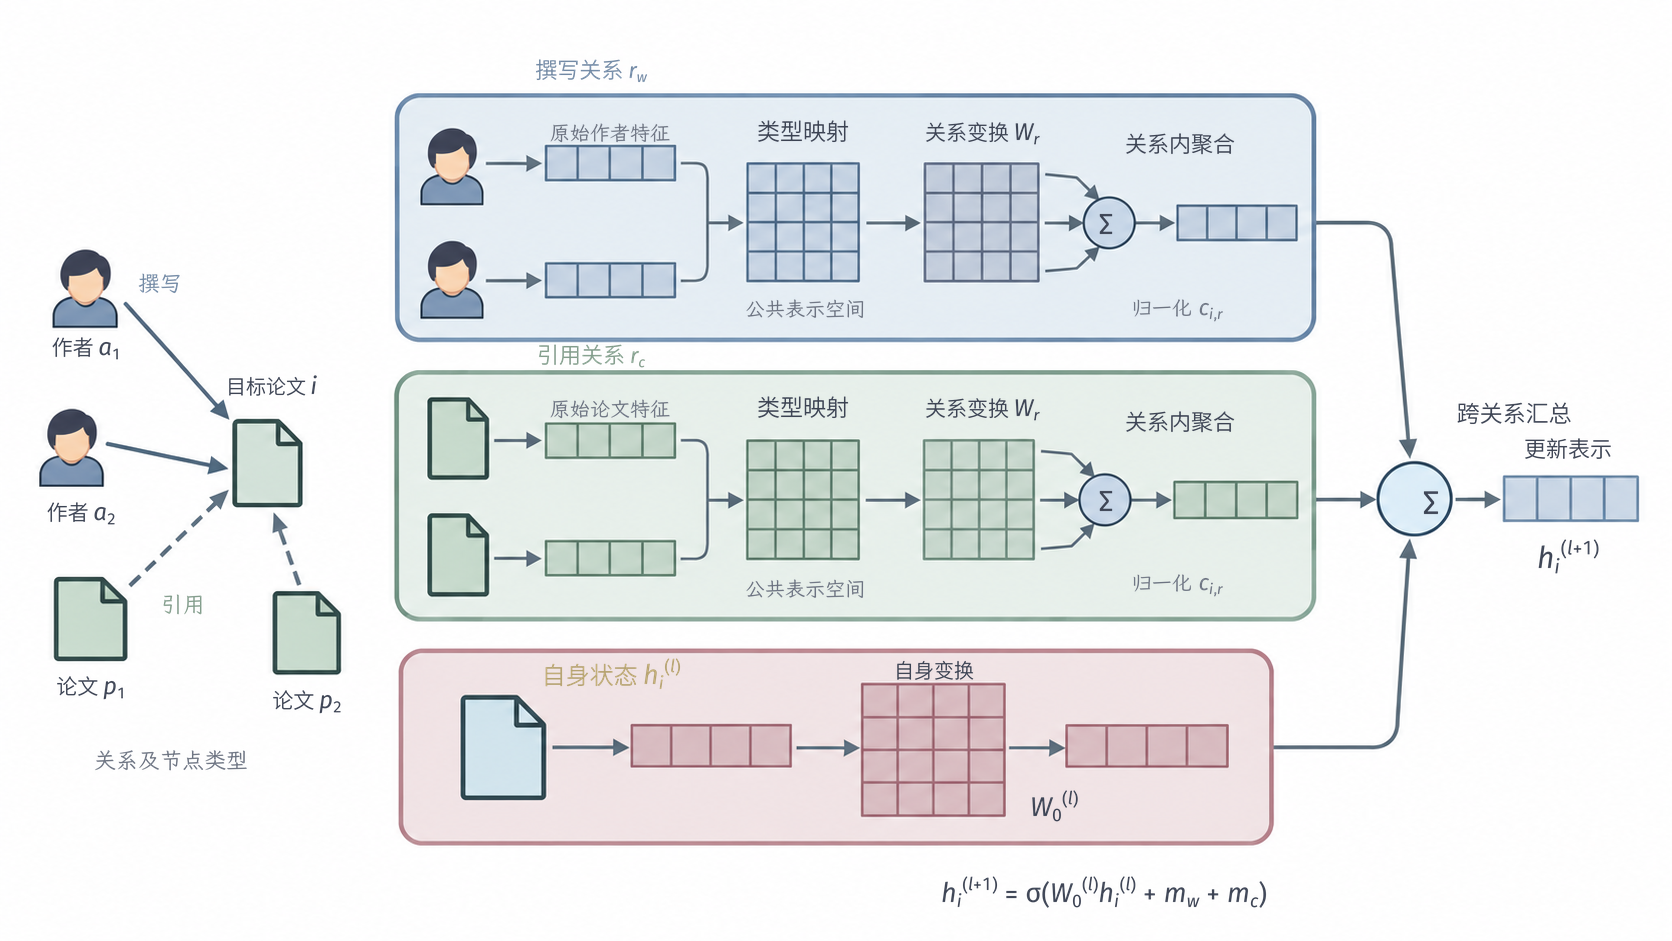
\includegraphics[width=141.563mm]{figures/08-neural-network-models/00-shared/generated/gnn-typed-relations/figure.png}
  \caption{两类节点与两种关系的消息组织。作者的撰写关系和论文的引用关系分别经过类型映射与关系变换，再在各关系内部归一化聚合；两路结果$\bm m_{\mathrm w}$、$\bm m_{\mathrm c}$与独立的自身状态路径汇总，形成目标论文的新表示。各类型的特征组表示同类节点，不表示提前求和；矩阵网格只示意变换，不声明实际维度。}
  \label{fig:gnn-typed-relations}
\end{figure*}
\FloatBarrier

\subsection{动态图}
\label{sec:gnn-dynamic}

社交互动、交易、设备连接都会随时间出现和消失，这时“固定图上传播十轮”和“现实中十个不同时刻”是两回事：前者是对\emph{同一个输入}做十次内部计算，后者是\emph{十份不同的输入图}。\term{动态图}（dynamic graph）把节点、边或属性随时间的变化也作为输入，模型既要处理当前关系，又要明确在做某个预测时哪些历史是合法可见的（不能用未来的边预测现在）。一种表示是\term{图快照}（graph snapshot）：在时刻$t$取得$\mathcal{G}_t$与$\bm{X}_t$，先在每张快照内用GNN编码当前邻域，再用循环状态沿时间累积。对持续存在的节点可写为
\begin{equation}
  \bm{z}_{i,t}=\operatorname{GNN}(\mathcal{G}_t,\bm{X}_t)_i,
  \qquad
  \bm{s}_{i,t}=\operatorname{GRU}(\bm{s}_{i,t-1},\bm{z}_{i,t})\text{。}
  \label{eq:gnn-snapshot-dynamics}
\end{equation}
这里$\bm{z}_{i,t}$包含当前图中的邻域信息，$\bm{s}_{i,t}$维护跨时间历史。节点身份用于对齐相邻快照中的同一个对象；新节点的初态、节点消失后的状态保留与重现规则也要约定。快照间隔决定哪些短时事件被合并或遗漏。

另一种表示是带时间戳的\term{事件序列}（event sequence），例如第$q$个事件$(i_q,j_q,\tau_q,\bm{a}_q)$表示两个节点在时刻$\tau_q$发生互动。每个节点维护自己的记忆，在事件发生后更新相关状态。消息可以读取两端的事件前记忆、事件属性，以及距离该节点上次更新的时间间隔；不参与事件的节点记忆可以暂时保留。TGN以消息函数、消息聚合、记忆更新和时序表示等模块组织这一类计算\scite{rossi2020tgn}

预测互动是否发生时，应先用事件发生前的历史评分，再用实际发生的事件更新记忆。这样的先后顺序使评分只读取当时的历史，随后到达的事件再进入记忆。批量事件处理也要明确是否能读取同批中较早的事件；同一时刻事件的处理应采用约定的同时更新或已有先后关系，使事件次序对应实际观测含义。

图~\ref{fig:gnn-dynamic-before-update}把内部传播、观测时间与事件先后三种顺序分开。下半部的评分位于消息和记忆更新之前，正是避免把待预测事件提前写入历史的关键。

\begin{figure*}[htbp]
  \centering
  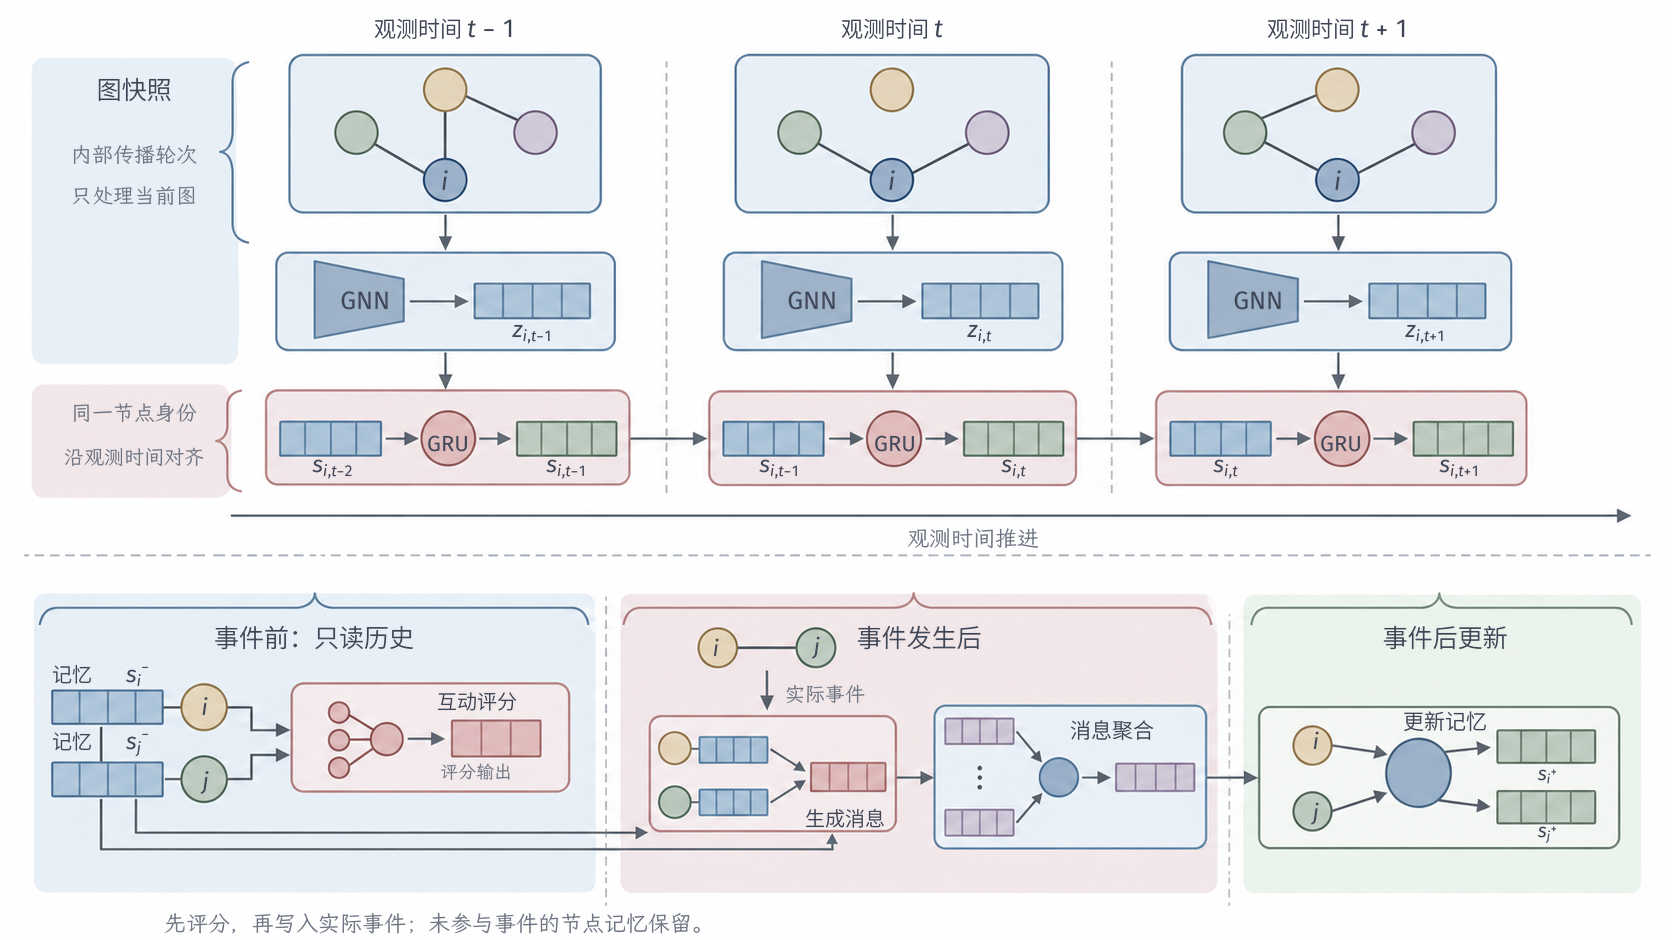
\includegraphics[width=141.563mm]{figures/08-neural-network-models/00-shared/generated/gnn-dynamic-before-update/figure.png}
  \caption{动态图的两种时间组织。上半部区分固定快照中的内部传播与同一节点沿观测时间的GRU状态演化；下半部先用事件前记忆评分，实际事件到达后才生成消息、聚合并更新参与节点。未参与事件的节点保留记忆。}
  \label{fig:gnn-dynamic-before-update}
\end{figure*}
\FloatBarrier

训练时可沿快照或事件展开反向传播，并在长流中按需要截断。评估未来事件时按时间划分，状态只由约定的可见历史推进；评估新节点时还要额外检查训练阶段是否已经接触其信息。内部传播深度、历史记忆长度和观测时间间隔共同影响计算，但衡量的是三种不同范围。

\subsection{高阶关系}
\label{sec:gnn-higher-order}

普通图的一条边只能连接两个节点，但现实中常有“一件事同时涉及多个对象”：一次三人合著、一笔多方交易、一个化学反应中多个反应物共同参与。如果把这样一个$k$元关系硬拆成所有两两配对的边，就无法区分“一次三人合作”与“三次各自的两人合作”——拆成的成对边集合可能完全相同。\term{超图}（hypergraph）用\term{超边}（hyperedge）直接表示一次连接多个节点的关系，把完整的参与组保留下来。记$\mathcal{H}=(V,\mathcal{E})$，其中$\mathcal{E}$是节点子集的集合；一条超边$S_a\subseteq V$就保留这次关系的完整参与组。

图~\ref{fig:gnn-hyperedge}展示一种计算表示：先让节点向超边聚合，再让超边把结果传回参与节点。将每条超边作为额外对象，会得到节点与关系对象构成的二部图；超边属性及非线性变换可以放在中间状态上。
\begin{figure*}[htb]
  \centering
  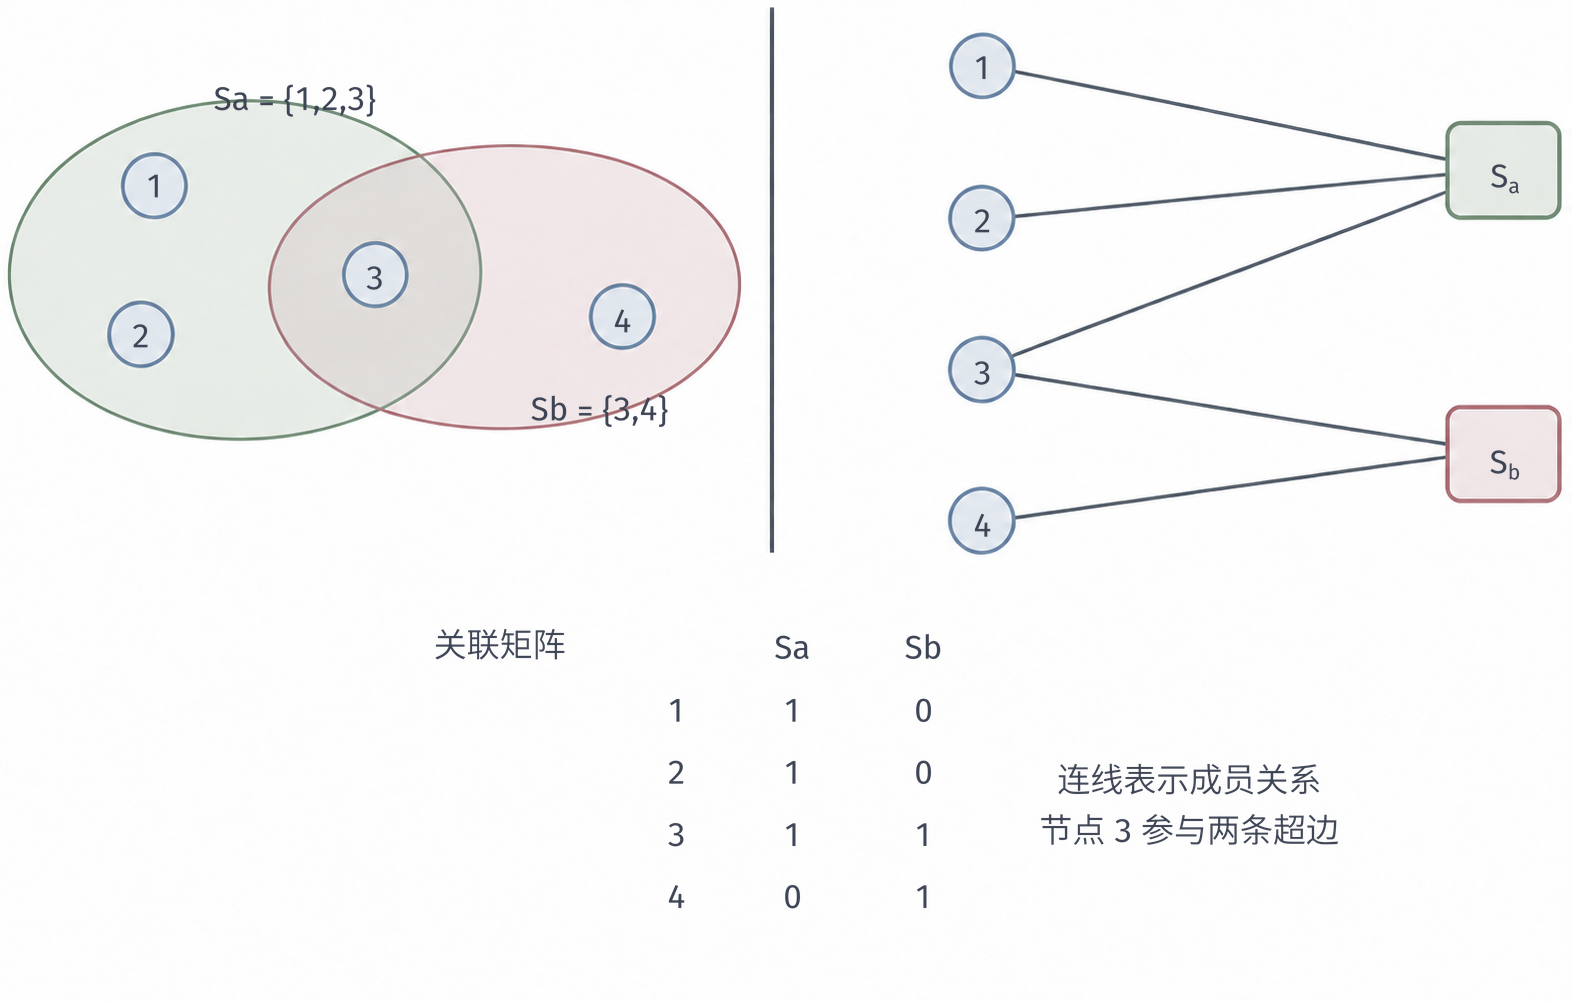
\includegraphics[width=133.096mm]{figures/08-neural-network-models/00-shared/generated/gnn-hyperedge/figure.png}
  \caption{超边及其关联表示。左侧一条超边$S_a$连接节点1、2、3，另一条超边$S_b$连接节点3、4。右侧将超边画成方框，以连线表示参与关系；下方$4\times2$关联矩阵用同一组0／1关系把“集合、二部图、矩阵”对应起来。方框保存关系状态，原始参与者仍由圆形节点表示。}
  \label{fig:gnn-hyperedge}
\end{figure*}
\FloatBarrier

令\term{关联矩阵}（incidence matrix）$\bm{B}\in\{0,1\}^{n\times h}$记录节点是否属于超边，$h=|\mathcal{E}|$，$\bm{B}_{i,a}=1$表示$i\in S_a$。设超边权重为$w_a>0$，$\bm{W}_e=\operatorname{diag}(w_1,\ldots,w_h)$，节点度$d_i=\sum_a\bm{B}_{i,a}w_a$，超边大小$s_a=\sum_i\bm{B}_{i,a}$。对非空超边及非孤立节点，一个归一化的传播为
\begin{equation}
  \bm{H}'=\sigma\!\left(
    \bm{D}_v^{-1/2}\bm{B}\bm{W}_e\bm{D}_e^{-1}
      \bm{B}^{\top}\bm{D}_v^{-1/2}\bm{H}\bm{\Theta}\right)\text{，}
  \label{eq:gnn-hypergraph-layer}
\end{equation}
其中$\bm{D}_v=\operatorname{diag}(d_i)$、$\bm{D}_e=\operatorname{diag}(s_a)$，$\bm{\Theta}$是特征变换矩阵。HGNN采用了这一类归一化超图卷积\scite{feng2019hgnn}

从右向左看，先由$\bm{H}\bm{\Theta}$变换节点特征，右端$\bm{D}_v^{-1/2}$再把发送节点$j$的表示除以$\sqrt{d_j}$。$\bm{B}^{\top}$将这些表示汇总到各条超边，$\bm{D}_e^{-1}$除以超边大小$s_a$，得到参与节点预缩放表示的平均值。随后$\bm{W}_e$把第$a$条超边的平均值乘以$w_a$，$\bm{B}$将这个结果送回该超边的全部参与节点，并把同一节点收到的各条超边结果相加。最左侧$\bm{D}_v^{-1/2}$再把接收节点$i$的结果除以$\sqrt{d_i}$，最后才施加激活。

因此，在激活之前，发送节点$j$的变换后表示$(\bm{H}\bm{\Theta})_{j,:}$对接收节点$i$的总传播系数为
\[
  \sum_{a:\,i,j\in S_a}\frac{w_a}{s_a\sqrt{d_i d_j}}\text{。}
\]
求和遍历同时包含$i$与$j$的超边；同一节点也会经其所属超边收到自身的贡献。这里按$s_a$求的是预缩放表示的组内平均，两端的节点度还会调整发送与接收尺度，整个节点传播不必是原始表示的简单平均。

我们可以沿图~\ref{fig:gnn-hyperedge}复核一次传播。取$S_a=\{1,2,3\}$、$S_b=\{3,4\}$，两条超边的权重均为$1$；作为教学算例，令单通道输入$\bm{H}=(1,2,3,4)^{\top}$、$\bm{\Theta}=1$，并使用恒等激活。节点度为$(1,1,2,1)$，超边大小为$(3,2)$。发送端预缩放后，四个节点的值为$(1,2,3/\sqrt{2},4)$；两条超边分别得到平均值$(1+2+3/\sqrt{2})/3$与$(3/\sqrt{2}+4)/2$。超边权重都为$1$，因此这两个平均值保持原值送回。节点3参与两条超边，将两个结果相加，再除以自身的$\sqrt{d_3}=\sqrt{2}$，得到
\[
  \bm{H}'_{3,1}
    =\frac{1}{\sqrt{2}}\left(
       \frac{1+2+3/\sqrt{2}}{3}
       +\frac{3/\sqrt{2}+4}{2}\right)
    =\frac{3}{\sqrt{2}}+\frac{5}{4}\text{。}
\]
这个结果把超边内平均、超边间累加和接收端缩放对应到同一次传播。

记录完整参与组后，还需要检查计算是否保留了这些组的差别。上述线性传播可以合成一个节点间矩阵（式\eqref{eq:gnn-hypergraph-layer}）。若两张超图产生相同矩阵，这一层也不能保留它们不同的组关系。任务依赖具体组时，可以在合成节点传播矩阵前保留超边状态、属性或组内非线性，使组关系继续进入输出。

另一类\term{高阶图网络}（higher-order graph neural network）把节点组作为状态对象，例如为节点对维护$\bm{h}_{i,j}$，使网络能够组合单节点状态难以保留的关系。它通过节点组索引安排状态与交互，可以由原图构造这些组，也可以读取已知高阶关系。Morris等将这种思路与高阶WL方法联系起来\scite{morris2019higherorder} 若显式维护所有$k$元节点组，状态数可达$O(n^k)$；选取部分子结构或局部组可以降低代价，但相应的区分能力也要重新说明。

\subsection{几何关系与对称性约束}
\label{sec:gnn-geometric}

在分子、点云这类数据中，节点除了连接关系还带有三维坐标。这里有一个比编号无关更严格的对称要求：把整个分子平移一下或在空间中转个方向，它的能量、毒性等\emph{标量性质}不应改变；而预测出的力、位移等\emph{向量}则应当跟着坐标系一起旋转。如果把绝对坐标直接喂给普通消息函数，网络就可能依赖“分子在空间中的绝对朝向”这种人为选择，违背物理对称性。几何图网络的做法是只在消息中使用\emph{旋转平移下不变的量}（如原子间距），需要输出向量时再乘以\emph{等变的相对方向}。

令变换后的输入坐标为$\bar{\bm{r}}_i=\bm{Q}\bm{r}_i+\bm{t}$，其中$\bm{t}\in\mathbb{R}^{3}$是平移，正交矩阵$\bm{Q}$满足$\bm{Q}^{\top}\bm{Q}=\bm{I}_3$。相对位移满足$\bar{\bm{r}}_i-\bar{\bm{r}}_j=\bm{Q}(\bm{r}_i-\bm{r}_j)$，距离$\lVert\bm{r}_i-\bm{r}_j\rVert_2$保持不变。用距离和其他不变属性产生标量消息，再用标量系数乘相对位移，就能构造等变的坐标更新。下面的撇号表示网络层的输出，因而$\bm{r}'_i$与变换后的输入$\bar{\bm{r}}_i$表示两种操作的结果。一个EGNN式的层可写为
\begin{equation}
  \begin{aligned}
    \bm{m}_{i\leftarrow j}
      &=\phi_e(\bm{h}_i,\bm{h}_j,
        \lVert\bm{r}_i-\bm{r}_j\rVert_2^2,\bm{a}_{i,j}),\\
    \bm{r}'_i&=\bm{r}_i+
      c_i\sum_{j\in N(i)}(\bm{r}_i-\bm{r}_j)\phi_r(\bm{m}_{i\leftarrow j}),\\
    \bm{h}'_i&=\phi_h\!\left(\bm{h}_i,\sum_{j\in N(i)}\bm{m}_{i\leftarrow j}\right)\text{。}
  \end{aligned}
  \label{eq:gnn-egnn}
\end{equation}
$\phi_r$输出标量，$c_i$是与坐标变换无关的归一化系数，$\bm{h}_i$此处由对所选欧氏变换不变的标量通道组成，边属性也具有相同不变性。EGNN使用距离构造消息，并用这种相对位移加权实现欧氏变换等变性\scite{satorras2021egnn}

证明只需跟踪各对象的变化。记$\bm{r}=(\bm{r}_j)_{j\in V}$为全部节点的坐标，$\bm{Q}\bm{r}+\bm{t}$表示对每个节点施加同一变换。以$\Psi$表示式\eqref{eq:gnn-egnn}中的坐标更新，把原输入的层输出记为$\bm{r}'_i=\Psi(\bm{r})_i$，把变换输入的层输出记为$\bar{\bm{r}}'_i=\Psi(\bar{\bm{r}})_i$；不变的节点特征、边属性和相应邻域暂时省略在$\Psi$的记号中。距离不变，所以消息及$\phi_r$不变；相对位移变为$\bm{Q}(\bm{r}_i-\bm{r}_j)$，整段坐标增量随$\bm{Q}$变换，加回$\bar{\bm{r}}_i=\bm{Q}\bm{r}_i+\bm{t}$后便有
\[
  \bar{\bm{r}}'_i
    =\Psi(\bm{Q}\bm{r}+\bm{t})_i
    =\bm{Q}\Psi(\bm{r})_i+\bm{t}
    =\bm{Q}\bm{r}'_i+\bm{t}\text{。}
\]
左侧先变换输入再执行层更新，右侧先对原输入执行层更新再变换输出，两种计算顺序得到相同坐标。变换输入后的标量层输出同时满足$\bar{\bm{h}}'_i=\bm{h}'_i$。邻接构造也须遵守该对称性，使整体变换前后的邻域对应，例如按距离阈值建边；若按固定坐标轴上的绝对位置选边，消息函数对称仍不足以保证整个模型对称。

正交矩阵还包括镜像反射。距离不变的模型因此可能无法区分互为镜像的手性构型；若目标会因镜像而改变，就需要只约束适用的对称群，并引入能保留相应方向关系的信息。所选对称群由目标决定：任务需要区分的方向关系应保留在输入与消息中。

若标量能量预测$\widehat E$可微且具有相应不变性，定义$\widehat{\bm{f}}_i=-\nabla_{\bm{r}_i}\widehat E$可以得到随旋转等变的力预测。具体地，由$\widehat E(\bar{\bm{r}})=\widehat E(\bm{r})$和链式法则，有$\bm{Q}^{\top}\nabla_{\bar{\bm{r}}_i}\widehat E(\bar{\bm{r}})=\nabla_{\bm{r}_i}\widehat E(\bm{r})$；$\bm{Q}$正交，故$\widehat{\bm{f}}_i(\bar{\bm{r}})=\bm{Q}\widehat{\bm{f}}_i(\bm{r})$。能量与力由同一可微函数联系，具有相应数学一致性；预测精度再由监督、构型覆盖和数值计算检验。

\section{理论分析}
\label{sec:gnn-theory}

与前几章一样，本节严格区分三个层面的问题：\emph{表达能力}问消息传递的结构是否\textbf{允许}网络区分目标所需的不同图（哪些信息在聚合中被不可逆地抹掉）；\emph{收敛性}有两个不同对象——参数能否被梯度下降\textbf{优化}到驻点，以及循环图网络反复迭代后状态能否\textbf{收敛}到唯一不动点；\emph{泛化性}问在\emph{独立的整图样本}上学到的规则对新图的风险。图结构既是帮助（强对称约束压缩了假设空间），也可能是限制（删掉了某些区分能力），下面保留结构区分能力、状态求值和样本边界的分析。

\subsection{表达能力}
\label{sec:gnn-expressivity}
\label{sec:gnn-propagation-theory}

表达能力问题在图上有一个特别干净的判别准则，可以一直追溯到消息传递的定义：\emph{如果两个节点（或两张图）在每一轮聚合后都得到完全相同的表示，那么任何只读取这些表示的读出都永远无法区分它们}。因此，要判断一个图网络能表达什么，只需检查在给定初始特征、聚合方式和传播轮次下，哪些不同结构会被“撞”成相同的表示。这里有两个层面的信息损失要分清：一是\emph{聚合函数}本身是否保留邻居的多重集（数量、内容），二是\emph{传播轮次和读出}是否保留了目标所需的结构关系。聚合若保留多重集、轮次足够、读出也保留所需结构，表达能力才可能达标；GIN正是通过把聚合和更新都设计成单射来逼近这条上界\scite{xu2019gin}。

\begin{theorem}[求和消息传递对度目标的表达与连通性目标的限制]
\label{thm:gnn-degree-connectivity-expression}
设节点初始特征均为$1$，图为无向简单图，最大度不超过预先固定的整数$D$。
允许保留邻居求和结果并接ReLU前馈读出，则一轮消息传递即可准确表示任意给定的节点度函数$g(\deg v)$。
但若各层只用共享节点更新和邻居多重集聚合，整图读出只使用最终节点表示的多重集，不加入节点标识或其他结构特征，则任何层数都无法区分六节点环$C_6$和两个不相交的三节点环$C_3\sqcup C_3$。对在两张图上分别取$1$与$0$的连通性目标，任意标量候选至少在一张图上有$1/2$的绝对逼近误差。
\end{theorem}
\begin{proof}
邻居特征求和恰等于度数。对有限整数$0,\ldots,D$指定$g$的值，分段线性插值可由ReLU读出准确表示。
两张环图则都有六个节点，每个节点有两个邻居。从相同初始特征出发，各轮节点都收到由两个相同向量组成的多重集，所以两张图的全部节点始终得到同一表示。整图读出相同，其输出不能同时距$0$和$1$小于$1/2$。
\end{proof}
求和能够保留数量信息，平均聚合在常数特征上却把不同度数都映为$1$。这解释了为何聚合方式直接影响候选空间。更强的GIN区分结论以单射更新与读出为条件，仍受相应图对的可区分性限制\scite{xu2019gin} 连通性反例针对上述消息传递族，并不覆盖加入高阶关系或结构位置特征的扩展。

\paragraph{反复传播对目标信息的影响：过平滑。}
\label{sec:gnn-oversmoothing}

多轮传播能扩大感受野，但直觉上也能想到它的副作用：如果每一轮都把节点的表示与邻居平均，那么传播很多轮之后，互相连通的所有节点都会被“搅”成越来越接近的同一个表示，节点自身的身份差异被逐渐抹掉。\term{过平滑}（oversmoothing）指的就是这种\emph{随深度增加、与区分节点有关的信息不断衰减}的现象；它不要求所有坐标严格相等才发生——只要任务所需的差异在各坐标尚未完全相等时就已经被削弱到无法利用，分类就会受损。值得注意的是，即便不同层使用不同参数，这种反复混合仍可能发生。

\begin{figure}[htbp]
  \centering
  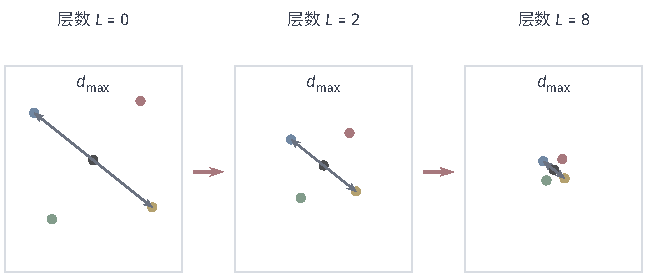
\includegraphics[width=109.580mm]{figures/08-neural-network-models/00-shared/tikz/gnn-oversmoothing/figure.pdf}
  \caption{过平滑的二维投影示意。五种颜色始终代表同五个节点，位置只是人为构造的表示投影，并非t-SNE实验；随着传播层数增加，点间最大距离缩小，节点身份仍在但可供下游区分的表示差异逐渐消失。过平滑描述的是任务相关差异受损，不要求所有坐标严格相等。}
  \label{fig:gnn-oversmoothing}
\end{figure}
\FloatBarrier

先看一个能够精确求解的简化模型：令激活与通道变换都为恒等，只反复计算$\bm{H}^{(l+1)}=\bm{S}\bm{H}^{(l)}$。假定非负无向图连通，并在每个节点加入正自环；对应$\bm{S}$具有唯一特征值1，其余特征值的绝对值小于1。定义单位向量
\[
  q_i=\frac{\sqrt{\widetilde d_i}}{\sqrt{\sum_j\widetilde d_j}}\text{，}
\]
则特征分解给出
\begin{equation}
  \bm{S}^L\bm{X}\longrightarrow\bm{q}\bm{q}^{\top}\bm{X},\qquad
  \lVert\bm{S}^L\bm{X}-\bm{q}\bm{q}^{\top}\bm{X}\rVert_F
    \leq\rho^L\lVert\bm{X}\rVert_F\text{，}
  \label{eq:gnn-linear-oversmoothing}
\end{equation}
其中$\rho$是其他特征值绝对值的最大值。证明依据是$\bm{q}$方向保持不变，其正交方向每次乘以绝对值至多为$\rho$的特征值。若图只有一个节点，就没有其他谱模式；此时约定$\rho=0$，从第一轮起传播结果已经等于$\bm q\bm q^{\top}\bm X$，式\eqref{eq:gnn-linear-oversmoothing}中$L\geq1$时的误差为零。

极限中，每个节点只剩同一个特征向量的度相关倍数；除以$\sqrt{\widetilde d_i}$后便相同。若图不连通，每个连通分量保留一个相应方向；若没有破除周期的条件，例如无自环的二部图，状态还可能振荡。这里的极限与速度由连通性、归一化和破除周期的自环条件共同支持。

真实GCN的非线性、学习权重及跨层连接会改变这一纯线性传播，式\eqref{eq:gnn-linear-oversmoothing}先说明反复混合的基本机制。Oono与Suzuki在特定激活及参数范数条件下进一步分析了表示靠近低维子空间的速度，说明传播谱与权重尺度需要联合考察\scite{oono2020oversmoothing} 低频聚合在有限深度可能有用，任务需要保留的差异被过度削弱时才构成问题。

残差连接可以为旧表示保留额外路径，跨层拼接或读出可以直接读取较浅表示，初始特征注入则持续补充原始节点差异。这些设计改变了反复纯混合的形式。若恒等分支加入后又与传播共同归一化，表示仍可能持续混合；残差实际保留多少差异，取决于完整更新。

\paragraph{窄通路对查询目标的限制：过压缩。}
\label{sec:gnn-oversquashing}

过平滑是“大家变得一样”，另一种困难则不同：远处\emph{确实有大量不同信息}要传过来，但通往当前节点的“通路太窄”，这些信息在瓶颈处被过度压缩、互相干扰，单个远处对象的影响被稀释到几乎无法辨识。\term{过压缩}（oversquashing）指大量关系信息沿有限条路径汇入有限维状态时，任务所需的远处影响难以有效传递。它关注的是远期影响\emph{通过哪些通路、汇入多大的状态}，Alon与Yahav从这一信息瓶颈出发分析了长程图任务\scite{alon2021oversquashing}。注意它与过平滑的判别方式不同：过压缩中各节点的表示并不一定趋于相同，真正的问题是单一输出对某个具体远端输入的敏感度趋近于零。

一个二叉树例子能展示具体机制。设每个内部节点只把两个子节点的标量取平均，深度为$k$的$2^k$个叶子为$x_j$，则根状态为$h_{\mathrm{root}}=2^{-k}\sum_jx_j$，根对单个叶子的偏导为$2^{-k}$。距离每增加一层，每个叶子的单独影响就减半，$k$层后衰减为$2^{-k}$；但根与各叶状态始终不同，所以这不是过平滑。图~\ref{fig:gnn-bottleneck}把汇聚树与图中“两组节点只能通过一条桥边通信”的情形对应起来。

\begin{figure*}[htb]
  \centering
  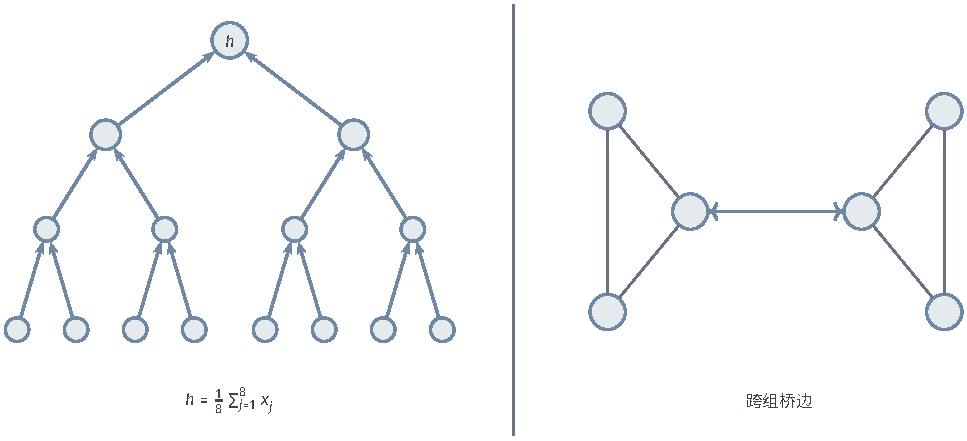
\includegraphics[width=163.791mm]{figures/08-neural-network-models/00-shared/tikz/gnn-bottleneck/figure.pdf}
  \caption{两种信息汇聚瓶颈。左侧八个叶子经三层平均进入一个根状态，每个叶子的影响系数为$1/8$；右侧两组节点的跨组信息必须经过一条桥边。图不要求所有状态相同，强调的是大量信息必须经过较少的表示通路。}
  \label{fig:gnn-bottleneck}
\end{figure*}
\FloatBarrier

若目标恰是叶子的平均，这种压缩就是所需计算；若目标要根据查询分别检索某个叶子，单一平均已经丢掉必要差别。因此，过压缩要相对于任务解释。压缩容量的分析需同时规定精度、噪声或连续性条件；无限精度实数与设备上的有限精度状态能够区分的历史数目不同。

增加状态宽度可以提供更多通道，增加传播轮次可以到达更远处，却也可能增加汇入同一状态的信息量。修改图结构、加入长程连接或全局读取，可以缩短路径并扩大跨区域通路；这些做法也改变了关系假设和计算量。残差主要保留已有信息路径，未必能解除一条桥边上的瓶颈。状态收敛、过平滑与过压缩因而需要分别诊断，再选择对应设计。


\subsection{循环状态的收敛}
\label{sec:gnn-convergence}

参数学习与状态求值是两个不同过程。有限轮消息传递直接定义输出，参数优化沿用第\ref{sec:ffn-convergence}节的相应条件；循环图网络若以不动点定义预测，则还需保证固定图、输入和参数下的状态迭代能够得到确定结果。


\label{sec:gnn-state-convergence}

不动点模型若迭代振荡或发散，就无法由极限确定预测。\term{压缩映射}（contraction mapping）给出充分条件：对同一输入，无论从哪两个初始状态出发，经过一次更新后它们之间的距离都按某个严格小于1的比例$c$缩小；在状态域完整且更新不离开该域时，反复迭代便趋向同一状态。这里的距离针对整张图的状态向量，消息聚合和所有节点的更新共同决定这个比例。

\begin{theorem}[收缩循环图网络的状态解唯一性与收敛速度]
\label{thm:gnn-state-solution}
固定图、输入与参数，若更新把非空闭状态域映回自身，并在同一范数下以非负统一比例$c<1$收缩，则任意该域内初态都趋于唯一状态$\bm h^*$，且
\begin{equation}
 \lVert\bm h^{(t)}-\bm h^*\rVert\leq c^t\lVert\bm h^{(0)}-\bm h^*\rVert\text{。}
 \label{eq:gnn-contraction-error}
\end{equation}
\end{theorem}
这给出了状态存在、唯一和迭代误差的结论；所用压缩映射结论可参考\BookChapterRef{chap:metric-spaces}{卷1《数学准备：计算、分析与几何》的“度量空间”章}。

在同一收缩条件下，相邻状态差还给出可检查的后验误差证书：对$t\geq1$，$\lVert\bm{h}^{(t)}-\bm{h}^*\rVert\leq c(1-c)^{-1}\lVert\bm{h}^{(t)}-\bm{h}^{(t-1)}\rVert$。$c$接近1时，误差证书中的放大系数较大，同一相邻差对应较宽的最终误差上界；迭代速度与停止容差由此联系起来。

例如采用矩阵状态更新$\bm{H}'=\sigma(\bm{S}\bm{H}\bm{W}+\bm{B}_x)$，其中$\bm{B}_x\in\mathbb{R}^{n\times m}$为固定输入项。若$\sigma$是$L_\sigma$-Lipschitz的，则Frobenius范数下
\begin{equation}
  \lVert\bm{H}'_1-\bm{H}'_2\rVert_F
    \leq L_\sigma\lVert\bm{S}\rVert_2\lVert\bm{W}\rVert_2
      \lVert\bm{H}_1-\bm{H}_2\rVert_F\text{。}
  \label{eq:gnn-state-lipschitz}
\end{equation}
乘积小于1且状态域不变时，可应用这一收缩结论。未经归一化的求和传播可能因最大节点度增大而放大该上界；对称归一化的无向GCN传播满足$\lVert\bm{S}\rVert_2=1$。门控中的门值落在$[0,1]$时，完整导数还包含门随状态变化的项，收缩条件需把它们一并计入。

收缩保证的是固定参数下的状态计算。参数更新会改变$F_{\bm{\theta}}$，训练目标通常仍然非凸。状态不动点让当前参数的预测器可以确定求值，训练进展和新样本误差再分别评价。收缩也是充分条件而非必要条件，有限轮次模型本来就不要求以不动点定义输出。


\subsection{泛化性}
\label{sec:gnn-generalization}

在图样本独立同分布、模型和损失满足相应约束时，复杂度或稳定性可以连接训练误差与新图期望误差，可参考\BookChapterRef{chap:deep-learning-theory}{卷3《基础、理论与可信性》的“深度学习的可学习性”章}。对分子属性预测，一张分子图及其标签才是一个样本，图内原子数不等于独立样本数；同一系统的连续快照或大图的重叠片段也未必独立。

单张图上的节点分类需要另按可见结构、标签依赖和数据划分评价。参数共享让同一更新规则能够用于更大的图，却不保证跨图规模、节点度或关系分布的预测误差不变。读出还要匹配属性：平均强调相对组成，求和保留数量累积，二者不能只按参数多少选择。

\section{常见应用}
\label{sec:gnn-applications}

下面三个任务的预测对象分别落在节点、边和整图层级，正好对应前面三种读出。贯穿它们的同一条纪律是：必须把\emph{可见关系、编码器、输出位置和监督标签}四者对齐——尤其要防止把“要预测的答案”通过输入或边泄漏给模型。这里展示一个完整模型如何接入任务，领域内的特征工程和评估协议留给应用卷。

\subsection{节点分类}
\label{sec:gnn-application-node}

以论文引用网络为例，每篇论文是节点，内容向量是$\bm{x}_i$，引用是有向边。若任务允许同时读取引用与被引用的信息，可以分别使用两个方向，或明确把图无向化；后一种选择会丢掉方向差别。内容编码器只使用约定的可见文本，类别标签另放在监督集合中。

下面的基本模型选择先把引用图无向化：只要两篇论文之间任一方向存在引用，就在编码图中保留一条无向边，记其邻接矩阵为$\bm A_u$。随后加入自环$\widetilde{\bm A}=\bm A_u+\bm I_n$，用$\widetilde d_i=\sum_j\widetilde{\bm A}_{i,j}$重新计算度，再构造$\bm S=\widetilde{\bm D}^{-1/2}\widetilde{\bm A}\widetilde{\bm D}^{-1/2}$。这样，后续使用的是前文的对称归一化传播算子；这里的邻居和跳数都指这张无向编码图。

一个基本模型是两层GCN：$\bm{H}^{(1)}=\operatorname{ReLU}(\bm{S}\bm{X}\bm{W}^{(0)})$，节点概率矩阵为$\bm{P}=\operatorname{softmax}_{\mathrm{row}}(\bm{S}\bm{H}^{(1)}\bm{W}^{(1)})$，Softmax逐行作用。按式\eqref{eq:gnn-node-loss}仅在训练节点上计算交叉熵，反向更新两层权重。两轮传播使每个预测可以读取两跳以内的内容与连接信息。

若要保留引用方向，可以按第~\ref{sec:gnn-relational}节的关系通路，为“引用”和“被引用”分别计算消息后再组合。此时传播规则要保留这两种通路，不能把原有向邻接直接代入上面的$\bm S$后继续使用无向对称算子的解释。

直推设定下，验证和测试节点的无标签特征与连接可以按协议参与编码；类别标签则保存在各自评估集合，训练只读取规定的监督标签。若预测未来发表的论文，则训练时不得使用未来引用边和文本，内容编码、建图及归一化也须按当时可见的信息重建。相同两层公式可以用于两种设定，但它们回答的是不同泛化问题。

还应比较只使用内容的前馈基线，以检查关系是否提供了额外信息。邻居类别常相近时聚合可能有用；关系跨越类别边界时，分开自身与邻居、处理方向或关系类型，可以保留类别边界两侧的不同信息，效果按实际引用与标签关系检验。

\subsection{连接预测}
\label{sec:gnn-application-link}

关系网络中，编码器先在可见图上产生$\bm{z}_i=\bm{h}_i^{(L)}$，解码器再为候选节点对评分。无向连接可用$s_{i,j}=\bm{z}_i^{\top}\bm{z}_j$；有向关系可用$s_{i,j}=\bm{z}_i^{\top}\bm{R}\bm{z}_j$，一般矩阵$\bm{R}$允许交换端点后得分变化。多关系任务可把$\bm{R}$改为类型相关参数。

训练批次包含已知正连接及从候选范围抽出的负样本，按式\eqref{eq:gnn-edge-loss}联合更新编码器与评分参数。未观察到的边并不一定是真实负例，它可能只是尚未记录；采样范围、正负比例和缺失机制决定目标的含义。

为区分总体比例与单个节点对的预测，考虑一个假设例子：正负标签都正确，现实候选中有$1\%$是真实正连接，训练却人为抽取相同数量的正、负例。现实候选的总体正例比例是$1\%$，训练采样分布中的总体正例比例是$50\%$；这两个数都不是每个候选节点对都应当输出的概率。对于给定的可见输入，二元交叉熵所要拟合的是训练采样分布下标签为正的条件概率，该概率还会随节点对的输入变化。Sigmoid输出是模型对这个条件概率的估计，有限样本、模型限制和优化误差都可能使估计偏离目标，使用Sigmoid本身不保证概率已经校准，即不保证在给出相同预测概率的一组候选中，正例频率就与该概率相符。

解释为现实候选中的实际连接概率时，需要处理现实比例与采样比例的差异，并核对负标记与真实连接的关系。若负样本只是未观察到的边，训练条件概率首先对应采样标签，缺失机制还会影响它与真实连接概率的关系；必要时应在匹配现实候选的数据上修正或校准。用于候选排序的得分与可直接按概率解读的输出，因此需要分别检验。

评估保留连接时，需要从编码图中移除这些边及其反向副本，避免编码器直接读取答案。训练正边是否在给该边评分时仍参与编码，也应说明；可以另外划分用于消息传递与用于监督的正边，或在批次中临时屏蔽目标边，使训练输入与目标评估口径对应。对未来连接，则先用历史图评分，事件发生后再更新动态图状态。

预测时对所需候选评分和排序。全部节点对数量为$O(n^2)$，即使编码器在稀疏图上计算，枚举全部候选仍可能昂贵。候选生成与负样本改变评价难度，比较模型时需要固定它们；随机负例与实际候选可能有不同难度，最终关系判断由部署候选上的相应指标检验。

\subsection{整图属性预测}
\label{sec:gnn-application-graph}

以分子属性预测为例，节点表示原子，边表示化学键。原子种类、形式电荷等作为节点属性，键类型等作为边属性，消息函数据此产生固定宽度向量。传播若干轮后，通过式\eqref{eq:gnn-readout}形成分子表示，再用前馈输出头预测标量，按式\eqref{eq:gnn-graph-loss}学习。输入编码、消息函数、更新与输出头共同接受梯度。

读出选择要与属性性质对应。随体系大小累积的量可以采用节点贡献求和的结构，强调整体分子组成；与规模不直接成比例的量可以使用平均或更一般的可学习读出。节点贡献求和编码了可加性的结构假设，局部表示能否充分表达真实属性仍需按任务检验。

只有二维连接关系时，网络不知道同一分子不同空间构型的坐标差别。若目标依赖三维构型，需要把预测时可得的坐标与几何关系纳入，并按第~\ref{sec:gnn-geometric}节处理对称性。近邻空间图传递空间接近关系，化学键图传递键连接；两种通路分别记录其输入语义。

训练和测试按完整分子划分；同一分子的多种构型或高度相近的结构是否跨划分，需要与目标使用场景对应。仅随机分图可能主要检查近似结构间的插值，按结构族划分则考察更远的迁移。验证图用于选择传播深度、宽度与读出，测试图用于评价相应设定下的预测误差。

\section{本章小结}
\label{sec:gnn-summary}

图网络用共享的消息函数处理数量可变、连接不规则的对象。邻居聚合与输入次序无关，并由共享更新形成节点表示，因此节点输出随编号置换而对应改变；对称的整图读出再消除编号顺序的影响。参数量可以不随节点数增长，计算量仍随图的规模与传播范围改变。

局部消息传递的$L$轮更新至多读取$L$跳邻居。谱滤波与邻域聚合提供两种描述，多项式滤波把相应谱响应落实为有限跳传播。度数归一化、邻居采样、内容加权和可区分的多重集聚合，分别改变信息组合的不同环节。

循环图网络还要区分有限轮展开与求取不动点；收缩条件保证的是状态求值，不能代替参数训练的收敛条件。多关系、动态、高阶和几何扩展则需要在消息中保留关系类型、时间、共同参与或坐标对称性。

聚合会限制结构区分能力。过平滑使反复混合后的节点表示趋同，过压缩则把大量远处信息挤入窄通路，两者需分别处理。新图误差还取决于独立样本、图的规模与度数、以及预测时可见的信息；直推、归纳和跨分布任务应采用与使用条件相符的数据划分。

\paragraph{扩展阅读}
Bishop与Bishop的教材及本章各类图网络原论文，可用于比较谱滤波与局部消息传递。教材中的统一计算视角与各模型的具体聚合、滤波和读出可以相互对照；置换对称、多重集区分及图级和节点级数据依赖，则对应本章的结构、表达与学习问题\scite{bishop2024deep}
